\documentclass[
  a4paper,
  abstract=true,
  twoside,
  listof=totoc,
  numbers=noenddot,
  bibliography=totoc,
  BCOR=1.5cm,
  headsepline,
  DIV=12,
  appendixprefix,
  final
] {scrreprt}

% You should select either american or british instead of english here:
\usepackage[ngerman,english]{babel}
\usepackage{fontspec}

\usepackage[citebordercolor={0.75 0.75 1},
filebordercolor={0.75 0.75 1},
linkbordercolor={0.75 0.75 1},
% pagebordercolor={0.75 0.75 1},
urlbordercolor={0.75 0.75 1},
pdfborder={0.75 0.75 1},
hidelinks,
plainpages=false,pdfpagelabels=true]{hyperref}
\hypersetup{%
  pdftitle={Leveraging core-local Resources to Prevent Side Channels in Trusted Execution Environments},
  pdfauthor={Pascal Scholz},
  pdfkeywords={TEE, confidential computing},
}
\usepackage[acronym, toc, nonumberlist]{glossaries}

\makeglossaries

% You can choose style "numeric" instead which is common in many papers.
% Without "maxbibnames=99" the bibliography entries only contain "First Name et al."
\usepackage[backend=biber,style=alphabetic,alldates=long,maxbibnames=99]{biblatex}

% FONT SETTINGS & ENCODING
% By default this build setup uses lualatex which supports special characters
% (öäüß<>) out of the box. If you ever want to switch to pdflatex but also
% keep the support for lualatex, add these three packages:
% \usepackage[T1]{fontenc}
% \usepackage[utf8]{luainputenc}
% \usepackage{lmodern}

\usepackage[nospace]{varioref}           % nice refs
\usepackage{csquotes}
\usepackage{graphicx}           % graphics
\usepackage{caption}            % manipulate fugures
\usepackage{subcaption}         % allow for subfigures
% Also checkout "minted" instead of "listings" - looks much nicer and supports
% more languages but requires "pygmentize" to be available on the command line
\usepackage{listings}           % nice source code listings
\usepackage{xcolor}
\usepackage{booktabs}           % nice tables
\usepackage{microtype}          % better looking text borders
\usepackage{siunitx}            % unified way of setting values with units
\usepackage{array}
\usepackage{fancybox}           % provide nice boxes
\usepackage{fancyvrb}           % algorithm-boxes
\usepackage{pdfpages}
\usepackage{hyphenat}
\usepackage{todonotes}
\usepackage{xspace}
\usepackage[mode=buildnew]{standalone}
\usepackage{tikz}
\usetikzlibrary{calc, snakes}
\usetikzlibrary{decorations.pathreplacing, arrows.meta}
\usepackage{setspace}
\usepackage{fancyhdr}           % enables cool header line and footer line manipulations
\usepackage{lastpage}           % enables the usage of the label "LastPage" to get the
% number of pages with \pageref{LastPage}

% use this one last
% (redefines some macros for compatibility with KOMAScript)
\usepackage{scrhack}

\addbibresource{own.bib}
\definecolor{mygreen}{rgb}{0,0.6,0}
\definecolor{mygray}{rgb}{0.5,0.5,0.5}
\definecolor{mymauve}{rgb}{0.58,0,0.82}

% Biblatex Style
\setcounter{secnumdepth}{3}     % limit enumeration depth
\setcounter{tocdepth}{1}        % limit TOC depth

% Listing Style

\lstset{ %
    frame=shadowbox,
    rulesepcolor=\color{blue},
    backgroundcolor=\color{white},   % choose the background color; you must add \usepackage{color} or \usepackage{xcolor}
    %  basicstyle=\footnotesize,        % the size of the fonts that are used for the code
    breakatwhitespace=false,         % sets if automatic breaks should only happen at whitespace
    breaklines=true,                 % sets automatic line breaking
    captionpos=b,                    % sets the caption-position to bottom
    commentstyle=\color{mygreen},    % comment style
    deletekeywords={...},            % if you want to delete keywords from the given language
    escapeinside={\%*}{*)},          % if you want to add LaTeX within your code
    extendedchars=true,              % lets you use non-ASCII characters; for 8-bits encodings only, does not work with UTF-8
    frame=single,                    % adds a frame around the code
    keepspaces=true,                 % keeps spaces in text, useful for keeping indentation of code (possibly needs columns=flexible)
    keywordstyle=\color{blue},       % keyword style
    language=C,                 % the language of the code
    % morekeywords={*,...},            % if you want to add more keywords to the set
    numbers=left,                    % where to put the line-numbers; possible values are (none, left, right)
    numbersep=7pt,                   % how far the line-numbers are from the code
    numberstyle=\tiny\color{mygray}, % the style that is used for the line-numbers
    rulecolor=\color{black},         % if not set, the frame-color may be changed on line-breaks within not-black text (e.g. comments (green here))
    showspaces=false,                % show spaces everywhere adding particular underscores; it overrides 'showstringspaces'
    showstringspaces=false,          % underline spaces within strings only
    showtabs=false,                  % show tabs within strings adding particular underscores
    stepnumber=1,                    % the step between two line-numbers. If it's 1, each line will be numbered
    stringstyle=\color{mymauve},     % string literal style
    tabsize=2,                       % sets default tabsize to 2 spaces
    title=\lstname                   % show the filename of files included with \lstinputlisting; also try caption instead of title
}

% Typesetting options
\tolerance 2414
\hbadness 2414
\emergencystretch 1.5em
\hfuzz 0.3pt
\widowpenalty=10000     % Hurenkinder
\clubpenalty=10000      % Schusterjungen
\vfuzz \hfuzz
\raggedbottom

% use nice footnote indentation
\deffootnote[1em]{1em}{1em}{\textsuperscript{\thefootnotemark}\,}

% ########################################################

% - Roman/Serif font for all headings.
%   Default is sans-serif which looks kind of unprofessional with the default font family.
% - Packages like titlesec don't work well together with KOMA
% - "disposition" means, that this setting is for all headings (chapter level, section level, ...)
%   see: https://mirror.physik.tu-berlin.de/pub/CTAN/macros/latex/contrib/koma-script/doc/scrguide.pdf
\addtokomafont{disposition}{\rmfamily}

% ########################################################
% With the fancyhdr package we can let all pages look more professional.
% Each page (except for special ones such as chapters or the cover) will contain a
% header that looks like this:
%
% Chapter %NUM%. %CHAPTER_NAME%                                                      3/10
%
% On even pages the page number is on the left, on odd pages the page number is on the right.
%
\pagestyle{fancy}
% Reset all existing header styles
\fancyhf{}

% Even pages (Ex)
% EL: even left: show page number
\fancyhead[EL]{\thepage~/~\pageref{LastPage}}
% ER: even right: show chapter
\fancyhead[ER]{\leftmark}

% Odd pages (Ox)
% OL: odd left: show page number
\fancyhead[OR]{\thepage~/~\pageref{LastPage}}
% OR: odd right: show chapter
\fancyhead[OL]{\rightmark}


% Additionally page number always on the bottom
% \fancyfoot[EC,OC]{\thepage}

% some common commands
\newcommand{\drops}{\texorpdfstring{\textsc{Drops}\xspace}{DROPS}}
\newcommand{\LLinux}{\texorpdfstring{L$\!^4$Linux}{L4Linux}}

\newcommand{\NOVA}{NOVA\xspace}
\newcommand{\QEMU}{QEMU\xspace}


% If you know when you will hand in your thesis, enter the date here.
\date{24. April 2025}
\newcommand{\printdate}{\@date}

\begin{document}

\pagenumbering{Roman}

\selectlanguage{ngerman}

\begin{singlespace}

  \subject{{\LARGE Diplomarbeit}}

  \title{Leveraging Core-local Resources to Prevent Side Channels in Trusted Execution Environments}

  \author{Pascal Scholz}

  \publishers{Technische Universität Dresden\\
    Fakultät Informatik\\
    Institut für Systemarchitektur\\
    Professur Betriebssysteme\\
    \begin{minipage}{\textwidth}%\\
      \vspace{6cm}
      {\normalsize }
      \begin{tabular}{ll}
        Betreuender Hochschullehrer: &
        Prof.\ Dr.-Ing.\ Horst Schirmeier\tabularnewline
        Betreuender Mitarbeiter:     &
        Dr.\ Carsten Weinhold\tabularnewline
        Betriebliche Betreuer:      &
        M.Sc. Thomas Prescher\tabularnewline
        & M.Sc. Sebastian Eydam
      \end{tabular} {\normalsize }
  \end{minipage}}

  \maketitle
\end{singlespace}

\cleardoublepage



\includepdf{images/diplom-aufgabe.pdf}
\cleardoublepage

\selectlanguage{ngerman}

\section*{\vfill{} \thispagestyle{empty}
  Selbstständigkeitserklärung}

Hiermit erkläre ich, dass ich diese Arbeit selbstständig erstellt
und keine anderen als die angegebenen Hilfsmittel benutzt habe.
\bigskip{}

\noindent Dresden, den \today\todo{Update date} % \printdate % if you defined date earlier
\vspace{2.5cm}

\noindent Pascal Scholz \cleardoublepage{}


% NOTE: if you selected british or american above, change that here too
\selectlanguage{english}

\begin{abstract}
% -*- Mode: Latex -*-

%  Zusammenfassung

% Zu einer runden Arbeit gehört auch eine Zusammenfassung, die
% eigenständig einen kurzen Abriß der Arbeit gibt. Eine halbe bis ganze
% DINA4 Seite ist angemessen. Dafür läßt sich keine Gebrauchsanweisung
% geben (für irgendetwas müssen die Betreuer ja auch noch da
% sein).
% - TEE important to protect code and data
% - Different technoligies allow for creation of TEE
% - Most are vendor specific extensions to processors, such as SGX and SEV-SNP
% - Other are optional, such as TrustZone
% - vendor locking as a result
% - Sie channel attacks pose a thread
% - Spectre/Meltdown effectively circumvent all security guarantees
% - Current work focuses on mitigating side channels used by transient execution attacks
% - no general solution
% - I propose an approach that uses a feature found in all commodity CPUs to detect the presence of side channels
% - for this i create a highly isolated execution environment
% - i show a design that allows for remote attestation using a tpm
% - i show what shortcomming my soltuion have and evaluate what constraints my isolation mechanism imposes to workloads
% - in the end, i evaluate my solutions regardning security to achive an argue why its not a feasable standalone solution with current available hardware

Trusted execution environments allow the execution of code in an environment
isolated from the remaining system and effectively aim to protect data against
unauthorized access and program code from being tampered with without detection.
To form a trusted relationship with the user, trusted execution environments
offer remote attestation, by which they can prove claims about the code running
inside of the environment and its state to the user.\\

Most hardware vendors offer special hardware extensions to allow the creation of
trusted execution environments. For commodity CPUs, these extensions are called
SGX and TDX in Intel processors, SEV-SNP in AMD processors, and TrustZone in Arm
devices. Vendors of these CPU extensions make a strong claim about their
security properties. With the advent of microarchitectural vulnerabilities in
2017, these claims have been proven by research to be broken or only held under
special circumstances. So-called transient execution attacks abuse the
microarchitectural behavior of modern CPUs. Software mitigations to certain
vulnerabilities exist but do not mitigate the source of the problems but rather
channels through which they extract information. Consequently, researchers
discover new vulnerabilities each year. \\

In this thesis, I develop a software-based approach to trusted execution
environments. Instead of using vendor-specific hardware extensions, my approach
is to use features present in nearly all commodity processors. By isolating a
single CPU core to run my environment, I create a highly isolated environment
that mitigates some of the attacks by design. For remaining attacks, I use
performance monitoring counters to detect data breaches. Together with this
isolation solution, I sketch a protocol that allows for remote attestation using
the Trusted Platform Module as a trust anchor and, therefore, allowing the
creation of a trusted execution environment without any vendor-specific hardware
extensions.\\

I show that this solution can reliably detect data breaches and isolate against
other forms of side-channel attacks. I also evaluate my prototype with regard to
what constraints it imposes on workloads. Finally, I will show that with the
currently available hardware, my solution can not alone protect sufficiently
from attacks and needs to be paired with additional solutions. I evaluate what
of the already existing solutions can be paired with my solution to increase
overall security properties.

%%% Local Variables:
%%% TeX-master: "diplom"
%%% End:

\end{abstract}

\cleardoublepage

\tableofcontents

\cleardoublepage

% remove this on final
\listoftodos
\cleardoublepage

\listoffigures
\cleardoublepage

\listoftables
\cleardoublepage

\pagenumbering{arabic}
% use \input for small stuff (like a list you include twice or a tiks figure)
% and \include for large latex compilation workloads (like a chapter) to get faster builds.
\chapter{Introduction}
\label{sec:intro}

% Die Einleitung schreibt man zuletzt, wenn die Arbeit im Großen und
% Ganzen schon fertig ist. (Wenn man mit der Einleitung beginnt - ein
% häufiger Fehler - braucht man viel länger und wirft sie später doch
% wieder weg). Sie hat als wesentliche Aufgabe, den Kontext für die
% unterschiedlichen Klassen von Lesern herzustellen. Man muß hier die
% Leser für sich gewinnen. Das Problem, mit dem sich die Arbeit befaßt,
% sollte am Ende wenigsten in Grundzügen klar sein und dem Leser
% interessant erscheinen. Das Kapitel schließt mit einer Übersicht über
% den Rest der Arbeit. Meist braucht man mindestens 4 Seiten dafür, mehr
% als 10 Seiten liest keiner.
\todo{Wenn's geklärt ist unbedingt die richtige Verwendung von We/I prüfen!}
\section{Motivation}
\label{sec:10:motivation}
Remote attestation is the ability of a trusted execution environment to prove claims about its state to an appraiser
over a computer network. \cite{coker_principles_2011} What first sounds like a solution to a rather abstract problem can
quickly prove helpful when considering the following example.
We find our example in the implementation of the automatic contact discovery of the Signal messenger. Signal itself is a
messenger that values the privacy of its users and the confidentiality of their communication. In doing so, Signal
implements a secure end-to-end encryption protocol to protect its users' chats.\cite{cohn2020formal}
To increase the user experience, Signal saw itself confronted by the problem of implementing a privacy-preserving way
for automatic contact discovery.\cite{SignalCd} The implementers were confronted with multiple problems. The first major
problem was the social graph. The social graph can either be centralized and stored on Signal's servers or decentralized
and stored on the user's phone. To minimize data stored on Signal's servers about their users, the implementers decided
to use the user's phone book. The second problem arises from this decision. The user's phone books must be processed so
that neither Signal nor their server operators can learn anything about the users.
To solve these problems, encrypting the phone books is not enough. For example, the user does not have any chance to
conclude from the communication alone with whom they are communicating. Even if the communication partner proves with
the help of signatures that they are the Signal server application, the user cannot verify what version of the server
application is running or if it processes the data as expected. Until now, we have not considered the server operator,
which might be malicious, too. They can manipulate and read the application's memory because they have privileged access
to the server's software and hardware. Such a powerful adversary could read decrypted secrets directly from
memory or modify the server application in a way that leaks secret data.
In this example, the user wants to verify that the Signal server application adheres to the following claims:
\begin{enumerate}
    \item The Signal server application executes the code the user expects
    \item The Signal server application is safe from being manipulated by privileged third parties
    \item Privileged third parties are unable to read the server applications' memory
\end{enumerate}
The server environment, therefore, needs a trusted security authority that can prove these claims to the users.
Additionally, hardware isolation mechanisms must protect this security authority against tampering attempts of
privileged third parties. Trusted execution environments solve this
problem by integrating two building blocks. First, they can execute code in an isolated execution environment.
Hardware enforces isolation, and interaction with the isolated code is only possible through defined interfaces of
the isolating hardware. This way, privileged software is not able to access memory-isolated code. Additionally, to
protect against memory bus-taping attacks, isolation hardware often encrypts the memory. The second building block
implements remote attestation. Through remote attestation, TEEs can verify that the execution environment runs the task
under hardware-assisted isolation protection.

If the TEE fulfills the aforementioned claims, it is safe to use. Moreover, most commodity CPUs currently
implement technologies that enable the use of TEEs. In that case, the CPU and its vendor act as
security authorities.\cite{tdx_whitepaper,kaplan_amd_2020,pinto_demystifying_2019,costan2016intel}
The story could be finished at this point if it was not the case that the respective CPU implementations contain bugs
that make it possible for attackers to circumvent their hardware-assisted isolation mechanisms and leak secrets through
side channels.\cite{kocher_spectre_2020,lipp_meltdown_2020,nilsson_survey_2020} While software updates could mitigate
specific side-channel attacks, the source of the information leaks is still persistent in hardware, with researchers
still finding new side-channel attacks each year.\cite{wikner2022retbleed,moghimi_downfall_2023,ragab_ghostrace_2024}
On the other hand, the example of Signal elucidates that proper working TEEs are important because they might process
critical data. It is, therefore, crucial to find a way to allow the execution of programs in a completely isolated and
side-channel-free environment.

\section{Contributions}
\label{sec:10:contributions}
As described in the motivation (see chapter~\ref{sec:10:motivation}) for this
thesis, we see a big problem in the general vulnerability by side channel
attacks on commodity processors. To fully exclude side channels, we propose
<Fancy Name\todo{think about a really fancy name}> to tackle the following
goals:

\begin{enumerate}
    \item We create an execution environment fully isolated from the remaining
          system by utilizing features found in all commodity CPUs. This means
          that we do not use any vendor-specific ISA extensions.
    \item We propose a TEE design to detect side-channel attacks and react
          appropriately.
    \item Our design ensures the usage of only core local resources. This means
          we implement a policy that is restricted to core local caches.
    \item We evaluate ways to enable such an execution environment to offer
          remote attestation features.
    \item We evaluate our implementation regarding system resources. In detail,
          we will evaluate what workload fits next to the local cache's runtime
          environment.
    \item We evaluate the TCB and against what attacker model our sole software
          solution can defend.
\end{enumerate}

With complete isolation and the exclusion of possible side channels, we aim for
a TEE solution that can withstand a wide array of possible attacks. Because of
time constraints in this thesis, we cannot implement a fully working TEE ;
instead, we can show the properties and concepts on a working proof of concept
implementation. We show that our solution can run next to a commodity operating
system such as Linux, implement communication channels through a well-defined
interface, and show that we can protect our implementation from being interfered
with by the commodity OS. Because we explore the technical feasibility, our
solution still depends on the commodity to install the environment.

\section{Structure}
\label{sec:10_structure}
In chapter~\ref{sec:state}, we will discuss technical Grundlagen that is important to follow the rest of the work. The first part
~\ref{sec:20:technical} we will discuss some details of the x86 microarchitecture. These details will allow us to understand the attacks
and what countermeasures to implement in the remaining parts of the thesis. Section~\ref{sec:20:tee} will then discuss the state of
the art by reviewing related work. In this, we will look at how trusted execution environments are implemented.
First, we will review hardware extensions followed by software solutions or software that enhances the security of
hardware extensions.

In chapter~\ref{sec:design}, I will explain the design of my implementation. In particular, we will explain in~\ref{sec:30:system} the general
design. In~\ref{sec:30:attacker}, we will revisit the attacker model and what design feature can be used to mitigate which attack.

Chapter~\ref{sec:implementation} will explain how I implemented the design proposed in~\ref{sec:design}. We will look at specific parts of
the implementation that are important to fulfill the security guarantees. Moreover, we will investigate what part
of the design was problematic to implement.

In chapter~\ref{sec:evaluation}, we will revisit the implementation described in chapter~\ref{sec:implementation}. We will evaluate the implementation in
chapter~\ref{sec:50:security} regarding how it protects against the attacker model described in~\ref{sec:30:attacker}. Moreover, we will evaluate
the practical use of our design in~\ref{sec:50:security}.

After we evaluate the implementation, we will look at missing parts and how to improve the implementation further. We
will do all of this in section~\ref{sec:futurework}, which gives an outlook on future work.

To come to terms with our results, we will give a short overview and summary of the results and findings of our work in
chapter~\ref{sec:conclusion}.


%%% Local Variables:
%%% TeX-master: "diplom"
%%% End:

\chapter{Background}
\label{sec:state}

% Hier werden zwei wesentliche Aufgaben erledigt:

% 1. Der Leser muß alles beigebracht bekommen, was er zum Verständnis
% der späteren Kapitel braucht. Insbesondere sind in unserem Fach die
% Systemvoraussetzungen zu klären, die man später benutzt. Zulässig ist
% auch, daß man hier auf Tutorials oder Ähnliches verweist, die hier auf
% dem Netz zugänglich sind.

% 2. Es muß klar werden, was anderswo zu diesem Problem gearbeitet
% wird. Insbesondere sollen natürlich die Lücken der anderen klar
% werden. Warum ist die eigene Arbeit, der eigene Ansatz wichtig, um
% hier den Stand der Technik weiterzubringen? Dieses Kapitel wird von
% vielen Lesern übergangen (nicht aber vom Gutachter ;-), auch später
% bei Veröffentlichungen ist "Related Work" eine wichtige Sache.

% Viele Leser stellen dann später fest, daß sie einige der Grundlagen
% doch brauchen und blättern zurück. Deshalb ist es gut,
% Rückwärtsverweise in späteren Kapiteln zu haben, und zwar so, daß man
% die Abschnitte, auf die verwiesen wird, auch für sich lesen
% kann. Diese Kapitel kann relativ lang werden, je größer der Kontext
% der Arbeit, desto länger. Es lohnt sich auch! Den Text kann man unter
% Umständen wiederverwenden, indem man ihn als "Tutorial" zu einem
% Gebiet auch dem Netz zugänglich macht.

% Dadurch gewinnt man manchmal wertvolle Hinweise von Kollegen. Dieses
% Kapitel wird in der Regel zuerst geschrieben und ist das Einfachste
% (oder das Schwerste weil erste).

In this chapter, I will provide background information on the topics revolving
around creating a standalone \gls{tee} that uses primitives of the processor
core to isolate itself. For this, I first introduce the basics about how x86
processor programming works in section~\ref{sec:state:technical}. Then we
revisit \glspl{tee} in general and how important building blocks look (c.f.
sections~\ref{sec:20:building_blocks} and~\ref{sec:state:tee}). We continue in
section~\ref{sec:20:attacks} to learn about side-channel attacks to later
understand vulnerabilities in existing \gls{tee} implementations.

\section{Technical Background}
\label{sec:state:technical}
This chapter gives us an overview of important mechanisms used by modern CPUs.
While there are other widely used architectures, such as Arm on mobile devices,
we explore these features in the example of the x86\_64 architecture. I decided
to do so because my proof of concept implementation targets the x86\_64
architecture, more precisely Intel's implementation of the \gls{isa}.

\subsection{Privilege Levels}
\label{sec:state:technical:priv}
The x86 \gls{isa} implements the following four privilege levels:
\begin{itemize}
  \item Level 0: \gls{os} kernel
  \item Level 1 and 2: \gls{os} services
  \item Level 3: User applications
\end{itemize}
Privileges granted by the processor increase with decreasing level, which means
that level 0 implies the highest privileges and level 3 the least amount. The
processor ensures that data can only be accessed by code that runs on a
privilege level that is higher than or equal to that defined for the data. All
four levels can be used together with memory segmentation. With paging, only one
bit is used to differentiate between privileged and unprivileged
accessibility~\cite{intel_sdm}. Moreover, only level 0 grants access to all
instructions available. For example, the \textit{WRMSR}, \textit{RDMSR}, and
\textit{HLT} instructions are included in the set of instructions only available
from level 0. For the remaining parts of this thesis, when I write about
\textit{privileged software} or \textit{system software}, I am referring to
software running at level 0. Whenever I write \textit{user space software} or
\textit{application}, I refer to code running at privilege level 3.

\subsection{Operation Modes}
\label{sec:state:technical:modes}
% The x86 architecture is rooted in the Intel 8086, designed in 1978. As a 16-bit
% microprocessor design, the Intel 8086 physically can only address 64 KiB of
% memory, which was enlarged by two segment registers to allow addressing nearly 1
% MiB of memory.
One advantage of the x86 \gls{isa} is its backward compatibility that allows
modern processor to execute code written for older CPU designs. To maintain
compatibility with legacy CPUs, over the course of time additional operation
modes were introduced to the \gls{isa}. Modern CPUs allow to execute 16-bit
legacy software in \gls{g_rmode}. The \gls{g_pmode} was introduced together with
memory protection to the x86 \gls{isa}. With x86\_64 the \gls{isa} is extended
by \gls{g_lmode}~\cite{intel_sdm}. To maintain the aforementioned compatibility
to legacy software, all x86 systems start in 16-bit \gls{g_rmode}. Because of
the limitation of the address space to the first 1 MiB of memory, code that
transfers a processor from \gls{g_rmode} to any other operation mode has to
reside in the address range of 0x500 to 0x7FFFF. This address range is called
low memory and is free for usage by system software.

% introduced an operation mode called
% \gls{g_rmode}. The name  originates from the fact that the 16-bit
% design used the real location in memory for addressing. The 32-bit operation
% mode of this CPUs is called \gls{g_pmode}, because it allows addressing memory
% through virtual addresses, allowing for memory protection. All x86 processors
% boot in \gls{g_rmode} to maintain compatibility to legacy software originally
% written for 16-bit CPUs. With the 64-bit extension x86\_64, AMD introduced an
% operation mode called \gls{g_lmode} that consists of two sub-modes called
% Compatibility Mode and 64-bit mode. Compatibility mode allows 64-bit system
% software to execute legacy 32-bit software. 64-bit mode extends the \gls{isa} by
% 64-bit operands and addresses, adds eight new general purpose registers and
% additional instructions. To use \gls{g_lmode}, system software has to prepare
% the processor by enabling additional processor features and creating required
% data structures.

\subsection{System Management Mode}
\label{sec:state:technical:smm}
Contrary to the operations modes described in
section~\ref{sec:state:technical:modes}, \gls{smm} does not activate additional
processor features. Instead, it is a hardware-assisted isolation mechanism that
protects firmware code from system software. In legacy systems, firmware used
the \gls{smm} to react to special hardware events that required the firmware to
react to platform events, e.g., energy management~\cite{intel_sdm}. The
\gls{smm} code resides in a specially protected area of the main memory,
referred to as \gls{smram}. \gls{smm} executes with privileges higher than level
0, and system software cannot interfere with it. In fact, \gls{smm} can
interrupt systems software whenever necessary, not vice versa. Firmware has to
issue a \gls{smi} to enter \gls{smm}.

\subsection{Virtualization}
\label{sec:state:technical:virt}
After Popek et al., a \gls{vm} is characterized by the following
definition:
\begin{quote}
  \textit{ A virtual machine is taken to be an efficient, isolated duplicate of
    the real machine. \\
  } \mbox{ -- Popek et. al. ~\cite{popek1974formal}}
\end{quote}
To allow the duplicate to run efficiently, a special environment is created that
enables the duplicate to use the resources of the real machine. To create this
environment, a piece of software called  \gls{vmm} is used. The \gls{vmm}
controls the resources of the real machine and ensures isolation between
duplicates and the real machine. To allow the \gls{vmm} to remain in control of
the real machine, a virtual environment is configured in a way that it traps
upon special conditions. These condition are, for example, access to memory or
the execution of instruction that would influence the real machine in a way,
that the \gls{vmm} could lose control over it. In such a case, control is
transferred back to the VMM. Processor architectures have to fulfill different
conditions to be called virtualizable. In the case of x86, additional \gls{isa}
extensions allow for virtualizability~\cite {adams2006comparison}. AMD
processors implement the Secure Virtual Machine (SVM) extensions while Intel
processors implement Intel Virtualization Extensions (VT-x or
VMX)~\cite{amd_manual, intel_sdm}.
inter-processor interrupt
\subsection{Interrupts and Exceptions}
\label{sec:state:technical:interrupts}
Interrupts and Exceptions are used to call system-specific functions and respond
to special conditions in the CPU or system. Exceptions are raised by the CPU
upon executing software or detecting hardware errors. Interrupts, on the other
hand, are either the result of software interrupt instructions or signals
generated by external hardware, such as keyboard input.
% Exceptions can be
% divided into three types by their origin or if they allow to restart the causing
% instruction:
% \begin{enumerate}
%   \item Faults: Result of an error with the instruction to execute
%   \item Traps: Result of breakpoint and software interrupt instructions
%   \item Aborts: The causing instruction cannot be restarted
% \end{enumerate}
Interrupts, can be divided into two classes:
\begin{enumerate}
  \item Maskable Interrupts: Masking an interrupt means that software can
    temporarily disable them. The interrupt controller holds them back until
    interrupts are enabled again.
  \item \Gls{nmi}: Software cannot turn off \glspl{nmi}. The interrupt
    controller delivers \glspl{nmi} to the CPU unless it currently serves
    another \gls{nmi}. When the CPU executes the IRET instruction in the
    interrupt handler, the interrupt controller can deliver the next \gls{nmi}.
\end{enumerate}

The x86 \gls{isa} assigns a vector number to each interrupt or exception. Vector
numbers range from 0 to 255 in newer implementations. The CPU uses the vector
number of an interrupt as an index to locate the respective handler function in
a data structure called the \gls{idt}. The \gls{idt} resides in the main memory
and contains the address of an interrupt handler routine for each vector. System
software defines the handler routines and writes their addresses to the
\gls{idt}. Once system software defines the handler routines, it makes the
\gls{idt} active by writing its address to the \gls{idtr}. System software
cannot write directly to the \gls{idtr} but has to prepare the special memory
descriptor from which the LIDT instruction loads the \gls{idt}. After setting up
and loading the \gls{idt}, the CPU executes interrupt handlers as defined by
system software. System software can enable maskable interrupts by executing the
\textit{STI} instruction. or disable them by executing the \textit{CLI}. \\

% Over time, interrupt controllers were improved and adapted to new use cases
% similar to CPUs. In \gls{g_rmode}, the CPU falls back to using the Intel 8259 or
% a compatible programmable interrupt controller (PIC), that delivers
% interrupts to the CPU. Once the PIC delivers an interrupt to the CPU, the system
% software must serve it and signal the PIC with an \gls{eoi}, that the serving
% routine is done. \\

\begin{figure}
  \begin{center}
    \includestandalone{images/lapic.tex}
    \caption{Illustration of how \glspl{lapic} integrate in a
    multiprocessor system (Figure after~\cite{amd_manual}, p. 1075)}
    \label{fig:state:technical:lapic}
  \end{center}
\end{figure}

In modern systems, multiprocessor configurations are prevalent, and each logical
processor core has its own Advanced Programmable Interrupt Controller (APIC).
Because the APIC is CPU local, these APICs are called local APICs or
\gls{lapic}. \glspl{lapic} forward interrupts from different sources to the
respective CPU core. For example, the \gls{lapic} receives interrupts such as
\glspl{ipi} from other \glspl{lapic} and forwards legacy interrupts from the PIC
via the LINT0 pin. CPU external devices can deliver their interrupts to the
IOAPIC, which forwards them to the respective \gls{lapic}. Devices that
implement PCI version 2.2 and later do not use the IOAPIC. Instead, these
devices use Message Signaled Interrupts by directly writing to a memory-mapped
register of the \gls{lapic}. Figure~\ref{fig:state:technical:lapic} shows a
schematic view of how the \gls{lapic} of each CPU core integrates into the
system. All \gls{lapic} registers are mapped to the 4-KiB \gls{lapic} register
space starting at the address specified in the \gls{lapic} base address
register. System software can then access \gls{lapic} registers with memory
reads and writes to the APIC register space. Most interrupts require the CPU to
interact with the \gls{lapic}. Exceptions are \gls{smi}, \gls{nmi}, INIT and
STARTUP \glspl{ipi}, as well as ExtINT. These interrupts are sent forwarded
directly to the CPU by th \gls{lapic}~\cite{amd_manual, intel_sdm}. \glspl{smi},
INIT and STARTUP \glspl{ipi} are not routed through the \gls{idt}. As described
in section~\ref{sec:state:technical:smm}, a \gls{smi} invokes the \gls{smm}.
INIT \glspl{ipi} transfer the CPU into a special state that effectively halts it
until it receives a STARTUP \gls{ipi}. All other interrupts are held pending by
the processor, and the CPU is reset to an initial state. The STARTUP \gls{ipi}
causes the CPU to begin processing a bootstrap routine, whose memory address
number is placed in the Vector field.

\subsection{Caches}
\label{sec:state:technical:caches}
% Since 1980, the performance growth of memory and processors has diverged
% steadily with an ever-growing gap. Hennessy et al. note a difference in
% performance growth of factor 1,000 for a single CPU core and memory
% technologies~\cite{hennessy2011computer}. To come by this disparity, CPU a
% on-chip buffer called cache memory.\\

% With processors gaining capabilities to
% process more and more data in parallel, for example by increasing the core count
% or introducing new instructions, the demand for fast memory further grows. For
% example, from November 2023 to January 2024, the number of systems in the TOP500
% list that employed CPUs with 96 cores per socket increased from 0 to 3, with the
% former maximum number of cores per socket being 72~\cite{top500}. To hide
% latencies and bridge the gap between CPU demand and actual main memory
% bandwidth, CPUs today employ fast local on-chip memory to buffer data they
% already accessed. If they reaccess this memory item, they can use these buffers
% to speed up access. This on-chip buffer described is called cache.\\

The cache is an integral component with the purpose of speeding up memory access
and organized in a multi-level hierarchy in modern CPUs. In this hierarchy, the
lowest and the nearest to the core level, called the L1 cache, implements the
fastest access. Most modern x86 CPUs divide their L1 cache into two parts: L1D
for data and L1I for instructions. With increasing levels, caches grow in size
but tend to be slower. For example, while the L2 Cache of AMD's recent Zen4 CPUs
offers only 14 cycles of latency, the L3 cache of the same CPU has a latency of
50 cycles~\cite{zen4}.\\

When the CPU tries to access data, it first queries the fastest cache. If the
CPU can locate the data in the cache, this is called a cache hit. On a cache
hit, the CPU can profit from reduced access time and improved bandwidth. The
opposite of a cache hit is called a cache miss, after which the CPU subsequently
queries the next level in the memory hierarchy. If it finds the data needed, the
CPU loads it into the nearest cache for faster access. Caches can only store a
limited number of items, organized in cache lines. Cache lines are a copy of the
main memory, and the processor uses this copy for all of its operations unless
otherwise configured. The processor loads data in cache line size granularity
from the main memory. All of this happens transparent to software and the
processor automatically manages its cache. \\

% Caches use the principle of locality, which consists of two kinds of locality.
% The first is called spatial locality. Spatial locality describes the observation
% that if a program accesses data from the main memory, data located at nearby
% addresses are the target of future accesses with a high probability. In this
% case, without any prefetching, the CPU tries to guess the size of the loaded
% structure to load parts missing in the cache in advance. If the CPU then
% accesses the neighbor of the first data, it already resides in the cache,
% lowering the latency. The second principle is temporal locality, which states
% that a program soon reuses memory references with a high probability. The CPU
% can, therefore, gain performance by storing recently used data in the cache for
% reuse.\\

With cache lines being copies of main memory items, and the possibility of
multiple copies of the same item existing in multiple caches at the same time,
the need for keeping them consistent arises. For this, different strategies for
writing data back to main memory exist:
\begin{itemize}
  \item \textbf{write-back}: Data modified in the cache is stored and written
    back to the main memory later. Cache coherency protocols are required to
    allow multiple devices to access the same memory range.
  \item \textbf{write-through}: The changes in the cache are instantly written
    to the main memory. These writes can slow down program execution because of
    costly main memory writes, but ensure consistency with system memory and
    cache content. This type is relevant for devices that access system memory
    but do not access CPU cache.
  \item \textbf{cache-disable}: The CPU cache is disabled, and the CPU
    performs all memory operations using the main memory.
\end{itemize}
% Legacy x86 software controls cache settings by setting or clearing configuration
% bits in the control register CR0. In a system employing modern x86\_64
% processors, systems software can set the caching strategy on page granularity
% (c.f. Chapter~\ref{sec:state:technical:paging}) by setting and clearing the
% respective bits in the page table entries. These settings are used in
% conjunction with values of the Memory Type Range Registers (MTTR) and Page
% Attribute Table (PAT) to calculate the effective caching strategy for a physical
% address.

Legacy x86 software has different ways of managing the cache settings than
modern \gls{os}. In modern \gls{os}es that use paging, the processor ignores the
write-through setting of CR0 and uses the page-level settings
instead~\cite{amd_manual}. The default in x86\_64 processors is to use a
write-back strategy.

\subsection{Cache coherence protocols}
\label{sec:state:technical:caches_protocol}
%An interesting difference in the x86\_64 implementation of Intel and AMD
%processors are the cache coherency and inclusion policies.
%AMD processors useMOESI as a cache coherency protocol~\cite{amd_manual}.
Intel processors
%,on the other hand,
use MESIF as a coherency protocol to maintain consistency of the caches among
different CPUs~\cite{thomadakis2011architecture}.
%MOESI and
MESIF is an extension of the MESI protocol, introducing the additional
\textit{Forward} state respectively.

The meaning of the states in the MESIF protocols are as follows:
\begin{itemize}
  \item \textbf{Modified}: The copy in the processor's cache is the most
    recent and modified. The copy in the main memory needs to be updated.
    Other processors in the system might maintain stale copies.
  \item \textbf{Shared}:  The copy is the most recent and correct copy of the
    data. Other processors may hold copies, too. Main memory holds the
    most recent and correct copy, too.
  \item \textbf{Exclusive}: The processor's and the main memory's copy are the
    most recent and correct copies. No other processor holds a copy.
  \item \textbf{Invalid}: The cache line is invalid and needs to be replaced by
    a valid copy from main memory or other CPU's caches before it can be used.
  \item \textbf{Forward}: Only one processor can hold a cache line in this
    state. Other processors might hold a correct copy of the cache line in
    shared state. The owning core responds to requests. The cache line is clear,
    so no writeback is required before discarding the line.
\end{itemize}

\begin{figure}
  \begin{center}
    \includestandalone{images/mesi.tex}
    \caption{MESI state transition of a cache line resulting from a (remote) activity (after~\cite{mckenney2010memory}, p. 4)}
    \label{fig:state:technical:mesi}
  \end{center}
\end{figure}

All cache lines are tracked to be in one of the states.
Figure~\ref{fig:state:technical:mesi} shows transitions of MESI states of a
cache line as a result from a core's own or another core's remote
access~\cite{mckenney2010memory}. The \textit{forward} state is essentially
equal to the \textit{shared} state when it comes to state
transitions~\cite{hay2012mesif}. It was created as an optimization to the MESI
protocol and reduces overhead in multi node
architectures~\cite{goodman2004mesif}. Important for my use case are the
following state transitions:

\paragraph{Foward from/to Shared}
Processor $0$ has the \textit{forward} copy of a cache line. Processor $1$
acquires a copy to read from processor $0$. Processor $1$ is the most recent
requester of the item and forwards it if any other processor requests a copy. It
holds the line in \textit{forward} state. Processor $0$ does not answer to
requests anymore, it now holds the cache line in the \textit{shared} state.

\paragraph{Exclusive to Shared}
Processor $0$ has the \textit{exclusive} copy of a cache line. Processor $1$
acquires a copy to read. In this case, the state of the line in processor $0$'s
cache changes from \textit{exclusive} to \textit{shared} to reflect that other
cores use the line.

\paragraph{Shared to Modified/Exclusive/Invalid}
Processor $0$ and processor $1$ both have the same data item in their local
caches. The state of both copies of the cache lines is \textit{shared}. Before
processor $0$ writes to the cache line it triggers the \textit{invalidation} of
the line in processor $1$'s cache. Upon receiving the acknowledgement of
\textit{invalidation} from processor $1$'s cache line, processor $0$ changes the
state of its cache line from \textit{shared} to \textit{exclusive}. At this
point the cache line is clean and matches the copy in the main memory.
Transferring a cache line to \textit{exclusive} can be done in preparation to an
anticipated write. After writing to the cache line, its state is changed to
\textit{modified}. If processor $0$ performs an atomic read-write operation it
will change its copy directly from \textit{shared} to \textit{modified}. The
state of the cache line in processor $1$'s cache is now \textit{invalid}.

Processors write back their data to the main memory once a cache line is evicted
or when other processors request the same data item. If another processor
requests the data item, then the owning processor will make the item available
via inter-cache transfers or through a writeback.

\subsection{Cache Inclusion Policies}
\label{sec:state:technical:caches_inclusivity}
On all current x86\_64 multicore CPUs, the \gls{llc} is shared among all cores
for synchronization and uses one of the coherency protocols. Older multicore
CPUs produced by Intel use an inclusive \gls{llc}, while more recent ones use a
non-inclusive \gls{llc}~\cite{intel_optimization, raptorlake_spec_sheet}. An
inclusive cache describes a cache containing the same content as lower levels
and vice versa. A line evicted, for example, in the \gls{llc}, is also evicted
in the lower levels. If an item is modified in a lower cache level, the changes
are automatically propagated to the higher inclusive cache
level~\cite{backes2019impact}. The opposite of an inclusive cache is an
exclusive cache design, as used by recent AMD CPUs~\cite{amd_z4_optimization}.
Exclusive caches do not replicate data in upper levels. Instead, the exclusive
cache level serves as a victim cache of the lower levels. Non-inclusive caches
can contain items of the lower levels, but inclusion is not enforced. This
means, if a line is evicted from higher levels its eviction is not enforced in
the lower levels~\cite{backes2019impact}.

\subsection{Hardware Performance Monitoring Counters}
\label{sec:state:technical:hpc}
\glspl{pmc} are registers that increment on the occurrence of predefined
microarchitectural events. The x86\_64 \gls{isa} specifies four freely
programmable general purpose \glspl{pmc}~\cite{amd_manual}. Concrete processor
implementations can offer additional counters. Similarly, the \gls{isa}
specifies architectural events that must be present in every processor
implementing x86\_64. Additional events are vendor and implementation-specific.
The four general purpose counters can be programmed to count any event supported
by the respective processor implementation. Vendors of x86 CPUs publish what
processor supports what additional events in their manuals. Moreover, a CPU
reports what events it supports in the result of the \gls{g_cpuid} instruction.
\\

In x86 hardware, performance counters are implemented by a set of two
\glspl{msr} per counter. One \gls{msr} can be programmed by system software with
the event to measure, while a second \gls{msr} counts the occurrence of the
respective event. Reading \glspl{pmc} can be done with the privileged RDMSR
instruction or from user space with the RDPMC instruction. In this way, a
program can poll the values of counters. The system software can also program a
threshold for a \gls{pmi}. Once the \gls{pmc} values exceed the threshold, the
\gls{pmi} is triggered, offering an alternative to expensive polling
techniques.\\

When using hardware \gls{pmc}, one must use the proper technique adopted to the
environment in which to obtain the counter values. Das et al. found in a
comprehensive survey that noise from the system is often present, e.g. context
switches influence the values of performance counters~\cite{das_sok_2019}.
Moreover, some counter events are over-counted while the CPU can undercount
others~\cite{weaver_non-determinism_2013}. It is therefore important to check
the right conditions for using hardware counters and verify that they work
correctly.

\subsection{Paging}
\label{sec:state:technical:paging}
% With the evolution of computer systems not strictly processing data in a batched
% manner anymore but instead allowing for multiple applications to run
% concurrently, a need for complex memory management arose. For example, system
% software must ensure that two applications programmed to use the same memory
% addresses do not influence each other. Segmentation is a legacy technique used
% in x86 systems to solve this problem. Segmentation allows the construction of
% address spaces that allow transparent translation of application addresses
% within an address space dedicated to the application. However, if applications
% do not entirely fit into memory, system software must perform expensive swapping
% operations between main and disk memory. In this swapping operation, programmers
% either need to split up their application into parts that must reside in the
% main memory simultaneously, or system software must swap the complete
% application.\\

% A solution to this is virtual memory implemented through
% paging~\cite{tanenbaum2015modern}.

The preferred way to manage memory in modern x86\_64 system is a technique
called paging. Paging splits the virtual address space into small, evenly
sized-parts called pages. The main memory is split into parts of the same size,
called page frames, by which each page can be backed.
% By splitting the address
% space into pages, system software can now perform swapping more fine-grained. If
% an application accesses a page not backed by a frame, hardware emits a fault,
% and system software can take the necessary steps to load it into physical
% memory. On the other hand, applications are now implicitly split into parts,
% allowing system software to only swap out parts of running applications.
% Additionally, paging allows applications to theoretically use the whole address
% space, with system software to decide what virtual address is currently backed
% by what physical page frame through its mapping function. This allows system
% software even to map a single physical page frame to the address spaces of two
% applications simultaneously, for example, if both applications use the same
% shared library. Knowing in detail how paging work on x86\_64 hardware will help
% understand content of later chapters.\\

% \begin{figure}
%   \begin{center}
%     \includestandalone{images/paging.tex}
%     \caption{Illustration of Virtual Address Translation with 4 Levels of Page Tables (after~\cite{amd_manual}, p. 597)}
%     \label{fig:state:technical:paging}
%   \end{center}
% \end{figure}
Hardware uses page tables that are hierarchically organized for the translation
of virtual to physical addresses. Each page table forms a level in the table
hierarchy and is the size of one page, storing references (addresses) to the
next lower level. The last page table in this hierarchy stores the address of
the physical page frame.
% By default, x86\_64 uses pages of size 4 KiB. Because
% x86\_64 uses 64-bit addresses, each 4 KiB sized page table can store 512
% entries. Figure~\ref{fig:state:technical:paging} shows the page translation of a
% virtual 64-bit address in x86\_64 with a page table hierarchy of four levels and
% a page size of 4 KiB. A virtual 64-bit address consists thereby of indices in
% the respective page tables to find the address as an entry in the lowest-level
% page table. Each page table in the hierarchy is referenced by its physical
% address.\\

% A virtual address for x86\_64 4-level paging with 4 KiB page size is divided
% into a 12-bit field used as an index in the page frame and four 9-bit fields,
% which the hardware uses as an index to access the content of the respective page
% level. The remaining address bits are sign extensions of bit 52, forming a
% canonical address. The hardware must perform a page table walk to resolve the
% virtual address.
% For the first step of a page table walk, the processor locates the address of
% the first page table, in this case, the PML4 table. The address of the PML4 is
% written by system software to CR3 after it created the page table. All page
% tables are aligned to 4 KiB, which leads to a value of 0 for the 12 least
% significant bits. Depending on the configuration, these 12 bits in CR3 are
% either used to determine the memory type of the PML4 or to store process-context
% identifiers.
To access the first table of the hierarchy, the CPU reads its physical address
from CR3.\\
% It uses the 9-bit index of the PML4 offset field in the virtual
% address to find the Page-Map-Level 4 entry containing the address of the next
% page table, the Page-Directory-Pointer table. The CPU accesses this table and
% all successor tables similarly until it locates the physical page. To access the
% data that belongs to the virtual address, the CPU uses the last 12 bits of the
% virtual address as an index to access the respective byte in the page frame. \\

% As the page table walk is expensive, the \gls{mmu} automatically stores the
% translated addresses in a cache called \gls{tlb}. System software has to manage
% page tables and \glspl{tlb} for each CPU independently. Furthermore, system
% software must maintain consistency between page tables and each \gls{tlb} by
% invalidating individual entries or the entire \gls{tlb}. If system software
% invalidates an entry, the CPU has to complete a page walk for this virtual
% address, upon which the \gls{mmu} updates the \gls{tlb}. Similar to other
% caches, filling entries in the \gls{tlb} works transparent to software. System
% software can use the INVLPG instruction to explicitly invalidate the \gls{tlb}.

\begin{figure}
  \begin{center}
    \includestandalone{images/pte_rights.tex}
    \caption{Layout of the 12 least significant bits in a page table entry (after~\cite{amd_manual}, p. 592)}
    \label{fig:state:technical:paging_rights}
  \end{center}
\end{figure}
The 12 least significant bits of each page table entry are used for management
properties, such as access rights management.
Figure~\ref{fig:state:technical:paging_rights} shows the layout of the 12 least
significant bits of a page table entry. The present bit is another property
stored in the 12 least significant bits of a page table's entry. It indicates if
the page the respective entry points to was initialized and loaded to the page
table. If this bit is clear, the CPU generates a \gls{pf} exception and expects
system software to load the respective entry. The CPU also generates a \gls{pf}
if software violates access rights. A second bit important for this thesis is
the Page-Level Cache Disable (PCD) bit. If the PCD bit is set, the CPU cannot
cache the respective page. Bit 3 (PWT) controls page-level write-through. If
system software sets this bit, the page table has a write-through caching
policy.

\section{Chain of Trust}
\label{sec:20:chain_of_trust}
Signatures of real humans differ because humans do not work entirely
deterministic. The process of forging signatures of other humans requires
dictations and practice by the forger because the human factor introduces
entropy to the process of signing. On the contrary, computers are built to work
deterministically. If the same input data is processed the same way, computers
working as intended by humans produce the same output. It is, therefore, that
authentication in the digital realm is implemented through cryptography and the
knowledge of secrets. Communication involves at least two parties, which we want
to call Alice and Bob in the following example.\\

When referring to cryptographic algorithms, a secret is called a key, and based
on the kind of keys used, we can differentiate between two kinds of
cryptographic algorithms. In symmetric algorithms, the same key is used for
encryption and decryption. Alice and Bob share thus the same secret. In
asymmetric algorithms, each of Alice and Bob maintain their secrets. These keys
have a public and a private part, respectively. Alice uses the public part of
Bob's key when they want to encrypt a message for Bob, and only Bob's private
key can decrypt a message in this way.\\

Digital signatures use asymmetric cryptography. Given that Alice wants to sign a
message so that Bob can verify that Alice is the sender, both proceed as follows
to fulfill their goal. First, Alice creates a pair of keys, a public and a
private one. Alice uses their private key to sign a message and distributes
their public key so others can use it to verify Alice's signature. To create
their signature, Alice first generates a pair of keys. Alice then published
their public key to make it available to Bob. When sending a message to Bob,
Alice uses a signing function that takes the message and the private key as
input and produces a signature, which Alice sends along the message to Bob.
Knowing Alice's public key, Bob can now check the validity of the signature with
the help of a signature validation function. This function takes the message,
the signature, and Alice's public key as input and generates the answer to
whether the message was signed with the signature.\\

Another problem arises when the network increases and Bob does not have the
chance to receive Alice's key in person. To prevent man-in-the-middle attacks,
Bob must ensure that the key they received over a network originates from Alice
and not from a malicious entity. The attack surface increases with the number of
different entities Bob wants to communicate with, as Bob needs to verify the
keys of each of their communication partner. A third party, the \gls{ca}, that
Bob trusts, can help with this. The \gls{ca}'s task is to pledge to Bob that a
certified key belongs to Alice or any other chosen entity and not a potentially
malicious third party. Bob trusts the \gls{ca} to do the keys' background check
and only deliver certificates of trusted identities. Alice first registers their
key with the \gls{ca}. The \gls{ca} own a pair of private and public keys too.
It uses these keys to cryptographically bind Alice's public key to their
identity. With this certificate, Bob can validate that a public key belongs to
Alice by validating the certificate with the \glspl{ca} public key. Alice now
delivers their public key and the certificate issued by the \gls{ca} to prove
that the key belongs to them. As long as the \gls{ca} is not malicious, Bob can
detect man-in-the-middle attacks if any malicious entity ships a key not
belonging to Alice. While all participants can create certificates for their key
with a dedicated key pair, such self-signed certificates could allow
man-in-the-middle attacks again. Hence, a trusted third party creates the
certificates.\\

\begin{figure}
    \begin{center}
        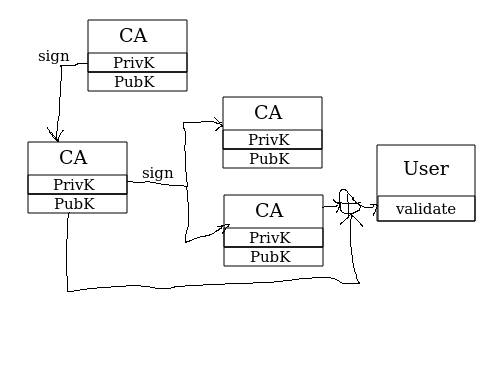
\includegraphics[width=.6\textwidth]{images/chain_of_trust_placeholder.png}
        \caption{Certifications in a chain of trust}
        \label{fig:state:technical:chain_of_trust}
    \end{center}
\end{figure}
\todo{This is a placeholder}

Because the single \gls{ca} is trusted by all participants in the network,
compromising it would mean control over all the communication in the network.
The solution to this is distributed trust. Multiple \gls{ca}'s can exist in a
network and compete with each other on the reputation gained from
users.\cite{perlman1999overview} Such a \gls{pki} is used in many network
technologies, such as HTTPS, that use the X.509 standard. Next to leaf
certificates issued to Alice and Bob, a \gls{ca} can also issue certificates on
keys that allow other entities to issue certificates and act as an \gls{ica},
creating a chain of certificates.
Figure~\ref{fig:state:technical:chain_of_trust} shows such a chain of
certificates. If Bob now wants to establish trust in the certificate provided by
Alice, they must first decide if they trust the \gls{ica}. The first step is to
verify that Alice's certificate was issued by the \gls{ica}. In the next step,
Bob needs to check all succeeding certificates until they reach the root
\gls{ca} by validating the \glspl{ica} respective certificates with the public
key of their issuer. In this way, Bob builds a chain of trust by verifying the
validity of the chain of certificates and deciding to trust the root \gls{ca}.
In the following section, we will see that such trust chains allow the
implementation of software attestation schemes.

\subsection{Remote attestation}
\label{sec:20:remote_attestation}
Remote attestation proves claims about a target
by delivering evidence to an appraiser over a network that supports these
claims. Before I further proceed to explain remote attestation, I want to
define the following terms similar to Coker et. al.\cite{coker_principles_2011}
\begin{itemize}
    \item \textbf{Appraiser}: Member of a network. Makes decisions about other
          parties on the base of delivered evidence.
    \item \textbf{Target}: Member of a network. Party about which properties the
          appraiser makes decisions.
    \item \textbf{Attestation}: Action of making claims about the target and
          delivering supportive evidence.
    \item \textbf{Measurement}: Collect evidence through direct and local
          observation
    \item \textbf{Attestation protocol}: Cryptographic protocol transmitting
          evidence about the claim. Trusted by appraiser
\end{itemize}

The appraiser and the target both follow orthogonal goals. While the appraiser
ideally wants to get as much information as possible about the target, the
target wants to preserve its privacy as well as possible and, therefore, conceal
as much information as possible. Both goals can be realized by employing a
trusted third party local to the target who can measure the target. This
third-party party then sends a signed report of the evidence on behalf of the
target. This report can contain the full raw measurement result, a reduced
variant, or a complete measurement substitute. For example, the reduced
measurement could be from a hash of the raw data. The substitute could be a
signature associated with the trusted third party that verifies that the target
fulfills the claims.

\subsection{Hardware Root of Trust}
\label{sec:20:hardware_root_of_trust}
A root of trust is defined by the Trusted Computing Group as follows:
\begin{quote}
    \textit{ A minimal set of system elements that have to be trusted because
        misbehavior is not detectable. \\
    } \mbox{ -- Trusted Computing Group\cite{tpm_architecture}}
\end{quote}

The Trusted Computing Group specifies that a hardware root of trust must be
available to enable remote attestation in a confidential computing
environment.\cite{tpm_architecture} A hardware root of trust is a device in a
computer system that the system can not manipulate. Moreover, it implements
security functionality such as encryption and random number generation. While
misbehavior is impossible to detect, hardware manufacturers can verify that
their devices work as intended by providing certificates. These certificates can
be embedded into the device with the help of tamper-resistant memory, such as
ROM or eFuses. A user can then check the validity of a certificate by consulting
the respective manufacturer's service. \\

Hardware roots of trust are necessary because system software could tamper with
software or memory to manipulate a possible software solution. The following
sections we review the most widely spread solutions to the hardware root of
trust. These implementations rely on dedicated hardware modules such as add-in
cards or unique, secure operation modes in CPU hardware. \\

\section{Trusted Execution Environments}
\label{sec:state:tee}

GlobalPlatform first used the term trusted execution environment to define a
solution for mobile trusted computing solutions.\cite{globaltee} Since then,
many definitions inconsistent and unspecific definitions have been published for
TEEs until the first precise definition was proposed by Sabt
et.al.\cite{sabt2015trusted}. They define the TEE in the following way:
\begin{quote}
    \textit{Trusted Execution Environment (TEE) is a tamper-resistant processing
        environment that runs on a separation kernel. It guarantees the authenticity of
        the executed code, the integrity of the runtime states (e.g., CPU registers,
        memory, and sensitive I/O), and the confidentiality of its code, data, and
        runtime states are stored on persistent memory. In addition, it shall be able
        to provide a remote attestation that proves its trustworthiness for third
        parties. The content of TEE is not static; it can be securely updated. The TEE
        resists all software attacks as well as physical attacks performed on the
        system's main memory. Attacks performed by exploiting backdoor security flaws
        are not possible. \\
    } \mbox{ -- Sabt et al.\cite{sabt2015trusted}}
\end{quote}

The first half of the definition describes a secure execution environment. A
secure execution environment can protect the integrity, authenticity, and
confidentiality of the application hosted by the SEE. Malicious privileged
software is thus neither able to modify the code, tamper with the runtime state,
nor observe code and data through the runtime. Contrary to TEEs, a SEE cannot
prove these claims against an appraiser, lest a third party outside the system.
This is because it does not require a root of trust to present in the system. To
prove its trustworthiness, TEEs employ remote attestation, which is the second
important aspect of the definition.\\

Trusted execution environment consists of several building blocks. The first
building block Sabt et al. propose is a secure boot. This building block allows
TEEs are used to verify that only a specific code of a particular state is
loaded. For a secure boot, a chain of trust is formed by verifying each
component's state. To generalize the secure boot requirement, a TEE must be
capable of verifying what code it loads to the environment. The second building
block is secure scheduling. Task executing in the TEE should not be able to
disrupt the main OS. Moreover, a TEE should implement means to allow
communication between the insecure world outside the TEE and the application
executing inside of it. Secure storage is one more building block. It allows the
application in the TEE to store data in a confidentiality, integrity, and
freshness-conserving way. Trusted I/O paths secure the communication between a
TEE and its users.

\subsection{TPM}
\label{sec:20:tpm}
\todo{A lot of passive to fix here}
The \gls{tpm} is a low-cost cryptographical coprocessor that offers different
cryptographic functions, such as hash functions, asymmetric and symmetric
encryption and decryption functions, asymmetric signing and verification
functions, and key generation functions. Implementations of the \gls{tpm} follow
different versions of specifications created and managed by the \gls{tcg}
consortium.\cite{tpm_architecture} The \gls{tpm} is specified by the Trusted
Computing Group as a system component with a state separate from the host system
on which it reports. The host system cannot directly manipulate the state of the
\gls{tpm} but has to use a defined interface to interact with the \gls{tpm}. To
separate the state between the host system and the \gls{tpm}, the \gls{tpm} is
implemented using dedicated hardware, such as a processor, RAM, ROM, and Flash
memory, all physically protected from the host system. Other physical separation
means can be used to implement \gls{tpm} services, such as unique processor
modes with dedicated memory access rights.\\

The most recent version of the \gls{tpm} specification is 2.0. The first
widespread family of \glspl{tpm} followed specification version 1.2, which was
implemented on modules shipped with personal computers beginning from the year
2005.\cite{arthur2015practical} One major drawback of version 1.2 was the
hard-coded usage of SHA-1 as a hashing algorithm. SHA-1 was first broken in 2005
by Wang et al.\cite{wang2005collision}. In 2011, NIST deprecated SHA-1 because
of security concerns.\cite{nist-sha1} \gls{tpm} 1.2 is constrained with respect
to its data structures to use either RSA or SHA-1\cite{tpm_architecture}
Therefore, when designing \gls{tpm} 2.0, the \gls{tcg} decided to leave the
exact algorithms specific \glspl{tpm} support open for their implementation.
Instead, the specification mandates a \gls{tpm} of version 2.0 to implement at
least one symmetric hashing, one symmetric encryption, and one asymmetric
encryption and signing algorithm. \\

In x86 systems, \gls{tpm} 2.0 is widely spread today and one of Windows 11s
system requirements. Often, \gls{tpm} is not implemented as a dedicated hardware
module but as firmware \gls{tpm}. The firmware \gls{tpm} is part of the Intel
Platform Trust Technology (Intel PTT) on Intel platforms. AMD platforms use an
implementation called fTPM, which is integrated within the platform security
processor.\cite{pirker2024brief} \\

While manufacturing, a vendor burns a \gls{ek} together with a certificate in
the \gls{tpm}. The \gls{ek} can be used to identify the \gls{tpm}, and the
certificate can be used to prove that the \gls{tpm} is genuine with the help of
the vendor's public key. Moreover, the \gls{tpm} uses the \gls{ek} as an input
to its key derivation functions. With the help of these key derivation
functions, a \gls{tpm} can generate keys for other applications such as
attestation, hashing, and signing. It never uses the \gls{ek} directly to
prevent leaking it in any form. A built-in entropy collector enables the
\gls{tpm} to generate random numbers. The \gls{tpm} uses hash functions to
generate a digest of input. Next to its cryptographic properties, the advantage
of a hash function is the output's constant length independent of the input's
length. Thus, the buffer only needs to be large enough to hold the result of the
digest. Message digests are used to store data outside of the \gls{tpm} or
generate certificates of values. The \gls{tpm} uses HMACs when storing data
outside of it. HMACs allow verifying that this data was not altered and
originates from a certain entity with the signing key.\\

The \gls{tcg} specifies two roots of trust for a trusted system. Two of them can
be implemented by the \gls{tpm}. The first is the root of trust for storage. The
\gls{tpm} implements memory that is shielded from the rest of the system, and
that can only be accessed by the \gls{tpm}. The second root of trust is the root
of trust for reporting. With its signing ability, the \gls{tpm} can attest to
values stored in its memory and create certificates for a measurement chain. The
third root of trust is the root of trust for measurement. This root is formed by
the CPU that measures on behalf of the system software or firmware. The
specification describes a core root of trust for measurement as the first
instructions executed in a new chain of trust, typically the firmware. In other
words, the core root of trust is trusted software that is believed to perform
the first measurement of the system correctly.\\

Software that performs the measurements instructs the \gls{tpm} to store its
result in \gls{pcr}. \glspl{pcr} are special registers of the \gls{tpm} that only
allow the \texttt{extend} operation and only reset when resetting the system.
The \texttt{extend} operation takes the current value of the \gls{pcr} and a new
value as input, concatenates both values, and processes the result with the help
of a hash function to create a digest that reflects the current system state.
The \gls{tpm} can assist in creating a chain of trust
(see~\ref{sec:20:chain_of_trust}) with the help of \glspl{pcr}. An example of how
to use the \gls{tpm} to build up a chain of trust is given by Arthur et
al.\cite{arthur2015practical} The system software can extend a certain \gls{pcr}
for each state before transferring control to the next application. The
application can then check the respective \gls{pcr} to contain a known good
value, indicating the platform was in a known good state before the application
was launched. If so, it can continue operation. If not, the application might
terminate. The measurement can also contain data about the application to be
launched to make sure that the application's integrity is not hurt. Remote
parties can use the \gls{tpm} attestation function to determine whether a system
was in a known good state at some time. For this, the \gls{tpm} offers the
possibility to sign the content of one or more \glspl{pcr}, producing a quote.
The remote party receives the quote, the public key, and the message contents.
The remote party can validate the certificate by executing the signature
validation function. With the public key of the \gls{tpm}, a remote party can
verify that the \gls{tpm} is genuine, and the vendor pledged to do so.
\todo{Do we need information on how system software interacts with the TPM?}

\subsection{Intel SGX}
\label{sec:20:sgx}
\todo{A lot of passive to fix here}
Intel SGX is an extension in x86\_64 processors manufactured by Intel, that
allows the creation of trusted execution environments. Intel first shipped SGX
in 2015, with processors implementing the Skylake microarchitecture. While
server-grade CPUs are still implementing SGX, Intel marked SGX was deprecated in
2021 in consumer-grade CPUs, beginning from CPUs implementing the Rocket Lake
microarchitecture. Costan et al. did an extensive study of SGX in 2016 and
documented in detail how SGX works and what it's security properties
are.\cite{costan2016intel} \\

Features of SGX include the creation of enclaves. Enclaves are especially
access-protected and encrypted system memory regions, with SGX preventing direct
memory access. In the creation process, memory pages are added to the enclave
page cache (EPC) and assigned to the enclave. Once assigned to an enclave, SGX
protects the memory page from unprivileged access, which includes all access
attempts not originating from the memory-owning enclave. After the system
software adds all pages to the enclave, it is marked as initialized. For the
initialization process, system software uses privileged instructions. After the
enclave is marked initialized, no more pages can be added to the EPC, and
interaction with the enclave is only allowed by using dedicated instructions
available only in user space. The EPC is similar to an inverted page table,
which purpose is to protect an enclaves security by ensuring the correctness of
the allocation process. SGX would, for example, refuse operation if it detects
that the same page frame was used for two different enclaves.\\

The enclave code runs at the permission level of
the application from which the enclave was called. Intel equips each CPU with
unique cryptographic keys that the CPU uses to encrypt code and data placed in
the EPC. These keys reside in memory made of electronic fuses that can not be
reprogrammed. Intel programs this memory in the factory process by burning some
of the fuses. Applications using SGX services do not necessarily need to run as
a whole in an SGX enclave. Because of restrictions on the size of the enclave's
memory, only parts of the data were handed to enclaves. Again, communications
between the enclave and user applications use special CPU instructions. In cases
where applications are split into parts residing in and outside of the enclave,
an application might want to verify the identity before sharing secrets. For
this, SGX implements local attestation.\\

As mentioned, SGX implements processor instructions dedicated to managing and
interacting with enclaves. Furthermore, SGX implementations create at least a
Launch Enclave signed by Intel. Third party enclaves that are not signed by
Intel require the Launch Enclave for successful initialization. It is necessary
in all cases when SGX is used.\\

An attesting enclave can verify its identity with another enclave in the same
system by generating a report. The attesting enclave calls the \textbf{ERPEORT}
instruction to generate this report. As a result, the CPU measures the attesting
enclave and generates a report that contains the measurement, the enclave's
identity, and a message provided by the enclave. The attesting enclave then
ships the generated report to another enclave for local attestation.
\begin{center}
    \begin{figure}
        \centering
        \includestandalone{images/sgx_attestation.tex}
        \caption{Software Attestation Scheme of SGX}
        \label{fig:state:tee:sgx_attestation}
    \end{figure}
\end{center}
Figure~\ref{fig:state:tee:sgx_attestation} shows the remote attestation scheme
implemented by Intel SGX. It extends the local attestation scheme so that a
third party not part of the system can verify the identity of an enclave. The
quoting enclave serves as a root of trust in this process. It is a unique
enclave provided by Intel that has access to the CPUs infused keys and can thus
act as a trust anchor. Upon receiving a report from another enclave, the quoting
enclave verifies said report and signs it. A remote third party can then check
the quoting enclave's signature to verify the correctness of the report..

\subsection{Confidential Virtual Machine Extensions}
\label{section:20:confidential_vms}
The goal of confidential Virtual machines is to protect the entire \gls{vm} from
the influence of a malicious hypervisor or other privileged software. Intel and
AMD offer individual \gls{isa} extensions for their processors to host
confidential Virtual Machines. Intel calls its solution Intel TDX, while AMDs
solution is called AMD SEV-SNP.\cite{tdx_whitepaper,kaplan_amd_2020} Both
solutions use the same fundamental building blocks to achieve the goals of
confidential \gls{vm}s. Misano et al. did a extensive comparison of both
technologies.\cite{misono_confidential_2024} Intel uses the SGX module for its
implementation. Additionally, to interact with a confidential \gls{vm}, the CPU
must be in the dedicated CPU operation mode called SEAM mode. Memory access is
only allowed in SEAM mode to protect confidential \gls{vm}s. Once in SEAM mode,
the CPU uses its Virtual Machine Extensions (VMX) capabilities to host and
interact with the \gls{vm}. For cryptographical features, such as signing and
key generation, Intel processors utilize the Intel Management Engine. The Intel
management Engine is a coprocessor located in the CPU package with special
firmware and a separate OS that is isolated from the remaining parts of the
system\\

For \gls{sev}, AMD uses the already implemented SEV capabilities and its
extensions. In its initial version SEV encrypts the memory of a virtual machine
with a dedicated key per virtual machine. SEV-ES extends the feature set by
additionally encrypting the system state, e.g. processor register, too. With the
most recent version, AMD introduced a feature called nested paging, which
manages an inverted page table similar to SGX to prevent attacks targeting the
\gls{vm}s page tables.\\

Unlike Intel's implementation, AMD processors do not utilize a dedicated CPU
mode but extend the existing \gls{vm} control structure by fields to enable
Secure Nested paging. For cryptography, the integrated AMD Platform Security
Processor, short PSP, is used. Both solutions encrypt the \gls{vm}'s memory to
protect the \gls{vm} from being manipulated by system software. While in Intel's
implementation, each \gls{vm} is encrypted separately, AMD's implementation
encrypts, once activated, the whole memory.\\

Both solutions use the trustee's knowledge of the initial state of the \gls{vm}
image. The assumption that the approach follows is that if the \gls{vm} is
started in a known state and protected from manipulation by the hypervisor or
other privileged software, then the \gls{vm} can be trusted in the following. To
follow this approach, a measurement of the initial \gls{vm} image is created and
cryptographically bound to the respective \gls{vm} instance through a message
authentication code. Before the trustee interacts with the \gls{vm}, they
request the \gls{vm} to verify its identity. For this, the \gls{vm} requests the
cryptographical hardware to sign a report. By signing the report, the
cryptographic hardware attests to its correctness and then hands it to the
trustee. The trustee trusts the implementation in the CPU and verifies the
signature of the CPU signed report. With this, the trustee knows if the \gls{vm}
images were expected. In the following, both the trustee and the \gls{vm}
exchange keys for further communication.\\

\subsection{ARM TrustZone}
\label{sec:20:trustzone}
As another widely spread ISA ARM dominates the mobile sector. Like x86, the ARM
architecture offers technology to allow isolated program execution. On ARM, this
technology is called ARM TrustZone. TrustZone is optional for ARM processor
implementations and slightly differs between the ARM Cortex-A application
processors and the ARM Cortex-M microcontroller-aimed processors. In the
following, we concentrate on the implementation of ARM application
processors. Pinto and Santos did an extensive survey of ARM TrustZone in 2019.
In their work, they describe technical properties of AMR TrustZone and how to
use it for the implementation of \glspl{tee} and hypervisors. Moreover they
explain technical details of Trustzone and review it's security properties
against other \glspl{tee}.\cite{pinto_demystifying_2019}\\

Conceptually, ARM TrustZone-enabled processors offer three processor operation
modes. The most privileged mode is the Secure Monitor mode or short SM mode. The
Secure Monitor mode is the mode in which the processor boots and the firmware
and Bootloader executes. The second most privileged mode is the Secure World.
This mode is intended to execute code isolated from the third and least
privileged mode, the Normal World. The Bootloader is responsible for installing
software intended to run in the Secure World. Isolation is achieved by hardware.
For example, the stack pointer (SP) and return address (LR) registers exist
twice to allow fast context switches between the Normal and Secure World. The
TrustZone Address Space Controller can be used to partition memory into regions
only accessible from the Secure World and those accessible by both worlds.
Changing between worlds can be done synchronously using the dedicated SMC
(System Monitor Call) instruction or asynchronously due to an interrupt. The SMC
instruction also triggers an interrupt. These interrupts are served by invoking
the SM, which decides upon its configuration if the interrupt received serves as
an entry point to the secure world. If so, the Secure Monitor invokes secure
world code to serve the interrupt.\\

ARM TrustZone does not specify the TEE and remote attestation features. Such
functionality has to be implemented by the code running in the Secure World and
might the implementation of those features might be specific to system or
hardware vendors. TEE and remote attestation functionality can be implemented by
a bare metal application or by using a trusted OS to host secure applications in
the Secure World. The first solution minimizes code size, while the second
offers the ability to host multiple applications in the Secure World. The
trusted OS would be responsible for isolating services running in the Secure
World against each other because applications running in the Secure World are
not isolated from other applications in the Secure World by hardware. Using a
trusted OS brings the downside of an increased trusted computing base compared
to a bare metal trusted application. TrustZone does not encrypt the memory of
the secure world, instead it utilizes the physical isolation of both worlds.\\

% \subsection{Security of Hardware Solutions}
% All hardware solutions isolate critical functions to protect them from being
% tampered with by privileged software. Because the \gls{tpm} protects only its
% state, I do not consider it when comparing the other hardware solutions. All x86
% solutions protect against adversaries that can tap the memory bus. These attacks
% become infeasible because all three solutions encrypt the memory content of the
% respective enclaves or \gls{vm}s. An adversary must break the respective cryptographic
% algorithms to inspect the memory content, as the processor decrypts the memory
% only once loaded. While an advisory cannot read the memory content, no solutions
% protect memory access patterns from recording. ARM TrustZone does not encrypt
% memory, so tapping the memory bus is possible. All solutions are vulnerable to
% side-channel attacks. Concerning the trusted computing base, ARM TrustZone
% relies conceptually on the functionally largest software stack. All x86
% solutions only rely on their respective implementation in the CPU SoC.
% Privileged software or firmware running in SMM cannot access the memory of
% enclaves or \gls{vm}s. On the contrary, ARM TrustZone relies on the Bootloader or
% firmware to install applications into the secure world. The processor's
% implementation does not protect the secure world application from being
% manipulated by the firmware. We could argue that ARM TrustZone's TCB is larger
% than that of the x86 solutions. As a side note, the x86 is a closed source but
% could be considered rather complex. The respective security processors on the
% respective x86 SoCs are running a small operating system themselves, making it
% hard to compare the TCB. Nevertheless, in the x86, the whole SoC implementation
% is manufactured by the same vendor, which the user ultimately has to trust.
% Contrary to this, in the ARM world, the user would have to trust the SoC
% manufacturer and the vendors of the Bootloader, firmware, and secure world
% application.\\

\section{Attacks on Trusted Execution Environments}

\subsubsection{Iago Attack Protection}
\label{sec:20:iago}
Checkoway et al. first published the class of Iago attacks in
2013.\cite{checkoway2013iago}. The attacker model in this attack class can
neither manipulate the application's code nor read the data from its memory. The
application is assumed to be unmodified and linked against unmodified libraries
but running on a malicious kernel. These application properties equal those of
SGX. The attack aims to manipulate the application through malicious system call
returns answered by the kernel. Such unexpected return values can cause the
application to work against its security interest or even manipulate the control
flow. SGX applications are potential targets for Iago attacks because they
depend on the runtime outside the enclave. Intel TDX and AMD SEV-SNP rely on an
untrusted hypervisor.\cite{tdx_whitepaper,kaplan_amd_2020} This untrusted
hypervisor could mount Iago attacks similar to malicious kernels. The WeSee
attack on AMD SEV-SNP, published by Schlüter et al. in 2024, shows that such an
attack is possible on AMD SEV-SNP by injecting specific interrupts into the
confidential VM.\cite{schluter2024wesee}\\

\subsection{Interrupt Based Side Channel Attacks}
\label{sec:20:interrupt_sca}
An attacker can learn about memory access patterns and behavior by using
interrupt-based side-channel attacks. The adversary in this class of attacks can
disrupt the execution of an enclave or confidential VM by sending interrupts.
These interrupts cause a context switch from the enclave or VM to the interrupt
handler of the OS or hypervisor. The malicious system software can then inspect
the state of the hardware, such as the L1 cache, the TLB, or the accessed or
dirty bits of pages. System software thus can single-step the enclave or VM with
a high enough frequency of malicious interrupts at instruction level
granularity. Attacks that utilize interrupts to learn about the state of trusted
execution environments exist for Intel SGX, ARM TrustZone, and AMD
SEV.\cite{van2017sgx, kou2021load, wilke2023sev}\\



\subsection{Transient Execution Attacks}
\label{sec:20:transientattacks}
In 2018, researchers published the Spectre and Meltdown
attacks.\cite{kocher_spectre_2020, lipp_meltdown_2020} These attacks were the
first to exploit the side effects of transient execution in modern CPUs and
affected all commodity architectures. For example, CPUs of the vendors AMD,
Intel, Qualcomm, and other ARM designs were affected. This class of new
transient execution side-channel attacks abuses the speculative execution
feature of modern CPU and defines an entirely new class of attacks. Furthermore,
they are the first class of attacks that abuse microarchitectural bugs. We
review this class of attacks in more detail as I aim to implement a TEE that
can defend against such an attack.\\

Modern CPUs use speculative execution to hide memory latencies. If, for example,
the control flow forks, the decision of which path to take often depends on a
value stored in memory. If this value is not persistent in the CPU cache, the
CPU needs to fetch the value from the main memory. While waiting for the result,
the CPU precalculates the most likely path. The CPU uses a dedicated buffer
called Branch Target Buffer (BTB) to decide what path to precalculate. The
Buffer records the n-th last paths taken, from which the CPU decides the most
likely path. If the value arrives from the main memory, the CPU checks its
decision and corrects its mistake, if any, to take the correct path. Overall,
speculative execution can lead to a huge performance increase. Older
publications see a performance increase from 27\% up to
87\%.\cite{espasa1997out, mock2005empirical}\\

In some cases, the decision about what path to precalculate is wrong. For
performance reasons, the CPU does not revert its microarchitectural state, like
cache content, on mistakes. Furthermore, if the wrongly speculatively executed
code produces an exception, the CPU does not serve it because the CPU should
never have executed the code path. Spectre and Meltdown-like attacks exploit
this design decision to read arbitrary memory. The attacker trains the BTB to
predict a path dependent on a memory address to prepare an attack. In the
training phase, the attacker uses valid addresses when the control flow
branches, which leads the CPU in the actual attack phase to predict that the
path in the training will be valid. In the attack phase, the attacker chooses an
arbitrary address. In preparation, the attacker evicts the value on which the
chosen path depends from the cache. Now, the attacker chooses a value that would
result in the decision to take a different code path. Because the attacker
trained the CPU before to take the now invalid path, it executes this one
speculatively until the requested value arrives. In the meantime, the CPU
executes a malicious read to the main memory using the address chosen by the
attacker. Later, the result of the malicious read returns and is stored in the
CPU cache. In the meantime, the CPU notices its mistake and takes the other
path. The value load resulting from the manipulated address still leaves traces
on the microarchitectural state of the CPU (in this example, the cache), and the
CPU does not throw an exception because the CPU should have never executed the
in this path. The attacker can now extract the secret through a side channel of
their choice. Because these attacks target microarchitectural behavior, a
complete redesign is necessary to fix the issue. Software mitigations are
available for specific attacks. For example, the Linux Kernel uses techniques
called retpopline and Kernel Page Table Isolation (KPTI) to mitigate Spectre
version 2 and Meltdown, respectively. On the other hand, software mitigations
can greatly impact performance, reaching from a 10\% to 800\% overhead,
depending on the workload.\cite{low2018overview} The class of transient
execution attacks is still highly relevant today, with at least five attacks
published in the last since 2023.
\cite{ormandy2023zenbleed,trujillo2023inception, moghimi2023downfall,ragab_ghostrace_2024, wilke2024tdxdown}
TEE solutions are affected, too, because these attacks enable attackers to read
arbitrary memory. The problem persists, and no solution exists to mitigate
transient execution attacks in general.\\



\cleardoublepage

%%% Local Variables:
%%% TeX-master: "diplom"
%%% End:

\chapter{Design}
\label{sec:design}

% Ist das zentrale Kapitel der Arbeit. Hier werden das Ziel sowie die eigenen
% Ideen, Wertungen, Entwurfsentscheidungen vorgebracht. Es kann sich lohnen,
% verschiedene Möglichkeiten durchzuspielen und dann explizit zu begründen,
% warum man sich für eine bestimmte entschieden hat. Dieses Kapitel sollte -
% zumindest in Stichworten - schon bei den ersten Festlegungen eines Entwurfs
% skizziert werden. Es wird sich aber in einer normal verlaufenden Arbeit
% dauernd etwas daran ändern. Das Kapitel darf nicht zu detailliert werden,
% sonst langweilt sich der Leser. Es ist sehr wichtig, das richtige
% Abstraktionsniveau zu finden. Beim Verfassen sollte man auf die
% Wiederverwendbarkeit des Textes achten.

% Plant man eine Veröffentlichung aus der Arbeit zu machen, können von diesem
% Kapitel Teile genommen werden. Das Kapitel wird in der Regel wohl mindestens 8
% Seiten haben, mehr als 20 können ein Hinweis darauf sein, daß das
% Abstraktionsniveau verfehlt wurde.

In this chapter, I will explain the design of the TEECore and how a system that
utilizes the TEECore prototype looks. The design tries to mitigate the risk of
covert side channels by fully excluding them on an architectural base.\\

In the first section (c.f.~\ref{sec:30:tee_general}), I will describe the
general system and usage of the TEECore prototype implementation. The second
section(section~\ref{sec:30:tee_kernel}) will explain TEECore in more detail and
how it tries to achieve its goals. TEECore alone does not implement any
workloads that third-party software can use. Such workloads and under what
constraints they must be implemented will be explained by
section~\ref{sec:30:tee_apps} of this chapter. I will then explain the remote
attestation scheme of TEECore in section~\ref{sec:30:tee_ra_scheme} before I
sketch the envisioned boot flow in section~\ref{sec:30:tee_boot_chain}. With all
components explained, I want to conclude this chapter by discussing the attacker
model that TEECore can defend and not defend against in
section~\ref{sec:30:tee_attacker_model}.

\section{General System Design}
\label{sec:30:tee_general}
In this section we will review how TEECore integrates in a system with other
components. Before we take a more detailed look on some of the components in
such a system, this section describes how system parts interact with each other.

\label{sec:30:system_overview}
\begin{figure}
  \begin{center}
    \includestandalone{images/30_system.tex}
    \caption{TEECore running in a system next to a commodity \gls{os}}
    \label{fig:30:tee_system_design}
  \end{center}
\end{figure}

Figure~\ref{fig:30:tee_system_design} shows an overview of a system integrating
TEECore next to a commodity \gls{os}. Speaking on a higher level, the bootloader
is responsible for partitioning the system into two parts: The first is managed
by TEECore, and the second is running the commodity \gls{os}. Because TEECore is
designed to run on the local CPU cache, the first partition consists of a single
CPU core. Thus, the remaining system resources, such as I/O ports, additional
CPU cores, and memory, are part of the second partition running the commodity
\gls{os}.\\

The design goal of TEECore is to enable the commodity \gls{os} to run workloads
in a shielded location so that no information can be leaked to other
applications. In figure~\ref{fig:30:tee_system_design}, such a workload is
defined as a trusted application.

TEECore uses a \gls{tpm} as a hardware trust anchor to store data and keys. It
utilizes measured boot to determine if the system is trustworthy when setting up
its services. Extend operations to the content of the \gls{tpm}'s \glspl{pcr}
form the backbone of TEECore's attestation feature and allow it to fulfill all
requirements of a \gls{tee}.\\

The second partition runs the commodity \gls{os} and all its applications. The
commodity \gls{os} implements system functions that allow applications running
on top of it to access services hosted in the partition running TEECore. The
commodity \gls{os} needs a special driver that implements the routines necessary
to communicate with TEECore and its services. Both partitions communicate via a
shared memory region. In the setup phase, this shared memory region is reserved
and placed into the memory map of both partitions for their systems to include
and map it.\\

The idea of partitioning the system is more similar to the idea behind ARM
TrustZone\todo{ref} than to \gls{sgx} or \gls{sev}. This is because TEECore
tries to use the given hardware's functionality to mimic an isolated trusted CPU
core and works more like the idea of a trusted world in ARM TrustZone instead of
\gls{sgx} and \gls{sev}. While AMD indeed integrates an ARM Core in their
\glspl{soc} and uses TrustZone to implement \gls{sev}, Intel uses a dedicated
CPU core based on a custom design to implement its Management Engine and
\gls{sgx} on top of it. TEECore's goal is to provide a solution for
x86 that allows the implementation of a \gls{tee} without using proprietary
vendor features.

\section{TEECore}
\label{sec:30:tee_kernel}
TEECore employs isolation mechanisms that protect data from being leaked while
protecting itself from modification by both the trusted application and the
commodity \gls{os} running on the rest of the system. For protecting TEECore
against malicious workloads, I use hardware-assisted domain separation through
different privilege levels, as widely used in other \gls{os}es. TEECore uses
\glspl{pmc} to observe the platform state and build protection measurements upon
those observations. The key component for this is hardware events that are
triggered when the CPU core under TEECore's control is forced to share data with
the remaining systems. Using respective interrupts, TEECore can react to these
leaks appropriately. I decided that the consequences of such a leak should lead
to a platform reset, effectively undermining an attack attempt. TEECore cannot
defend itself against Denial-of-Services attacks.\\

TEECore kernel utilizes CPU core-exclusive \gls{pmc} registers to monitor data
flow between cores for isolation. The assumption on this part of the kernel is
that shared parts of the CPU can be used to create a hidden channel for
transferring data. If the CPU uses such resources, for example, a shared L3
cache, then those effects trigger respective performance monitoring events. With
respectively programmed \glspl{pmc}, those events can be counted by the TEECore.
\glspl{pmc} can be programmed to emit a \gls{pmi}, which the \gls{tee} uses to
register forbidden events. Because the source of those events must be known to
conclude the presence of an attacker safely, only selected events can be used by
TEECore and the \gls{tee} must ensure its regular operation does not trigger the
respective events. TEECore, therefore, must ensure the use of local CPU
resources only. On Intel platforms, I use events that measure interaction with
the so-called offcore. Offcore events result from the core interacting with
resources that are not local. These events include reading/writing to shared
caches, RAM, or other components. From the fact that TEECore allows only usage
of core local resources, a memory constraint is the result, which confines the
size of usable memory to that of CPU local caches. Moreover, TEECore has to
ensure that it can detect access to data that is implicitly shared through cache
coherency in the inclusive L3 cache.\\

Before the TEECore can transfer control to tasks, it must bring the environment
to a defined state. All memory is stored in the CPU's local cache in the
exclusive or modified state. To achieve this, TEECore writes to all memory it
has to protect, invalidating shared cache lines in other cores in this process.
As a result TEECore can detect whenever a remote CPU accesses data from RAM or
shared L3 cache, as the remote copies the respective memory items to its L1
cache, triggering a MESIF state change in the isolated cores cache. To protect a
task against interrupt-based attacks, TEECore has to set up the \gls{idt}
correctly so that any occurrence of any interrupt results in a system reset.
TEECore achieves this by setting the \gls{idtr} to zero, which results in a
general protection fault once the CPU tries to locate the \gls{idt}. Because
this provokes a second fault after the first, the CPU generates a double fault,
ultimately resulting in a triple fault and, thus, a system reset. TEECore
triggers a platform reset when receiving maskable interrupt and \glspl{nmi} this
way. Furthermore, it programs the \gls{pmc} to detect attacks on itself or its
payload as soon as possible. TEECore uses the possibility to generate
\glspl{pmi} on the overflow of a \gls{pmc}. As explained, the resulting
\gls{pmi} leads to a system reset. Important at this point is the fact that
TEECore can only react to attacks in this way. It cannot prevent them
entirely.\\

External memory, such as the shared memory region and memory mapped registers of
the \gls{tpm}, are mapped as un-cacheable. One reason is that it prevents
external memory from polluting the cache. Another more relevant cause for this
is that TEECore can single out what offcore event was caused by malicious
interactions through specific events. For example, read or write requests served
by DRAM are allowed for these types of memory, while the same operations being
served by other CPUs are not allowed.\\

The payload of TEECore is called a trusted application. In the proof of concept,
tasks are implemented as functions and are thus statically embedded into the
TEECore binary. A trusted application is allowed to access the shared memory
communication channel. TEECore monitors this access and makes it part of its
measurements. After a trusted application run, TEECore creates a Snapshot from
the \gls{pmc} registers and a report based on this information.

\section{Trusted Applications}
\label{sec:30:tee_apps}
Trusted applications run in user space in the secure partition and provide
services to software in the normal partition. Compared to applications running
on top of a commodity \gls{os}, applications running in an environment managed
by TEECore must respect multiple restrictions.\\

For now, the design does not support the dynamic installation of user space
applications in the \gls{tee} environment. This restriction is the consequence of
TEECore not being a fully fledged \gls{os} and the missing availability of
\gls{os}-specific libraries such as a standard C library. As a result, an
application must be implemented as a function in the TEECore using the
respective framework. Changing the application requires the recreation of the
whole TEECore binary. While this reduces the flexibility of running systems, it
allows for easier integrity measurement of applications because they are
statically embedded in the TEECore binary, which is already measured in the boot
flow through the measured boot. Moreover, embedding the application in the
TEECore binary as a function removes the necessity to implement an executable
loader, which reduces the amount of code and, therefore, the size of the binary.
Another restriction is that the whole run time environment has to fit together
with the application into the CPU's local cache.\\

The small size of available memory also restricts the size of data the workload
can generate. Working with large data sets is not possible, as exceeding the
capacity of the cache will lead to replacements in the local cache, which will
result in leakage to a shared part of the memory subsystem, an event considered
by TEECore as an attack. TEECore then reacts similarly, which results in a reset
of the whole system. Moreover, the organization of cache structures can
influence memory usage. I will evaluate such effects in chapter\todo{hier die
Kapilnummer nennen}. The last aspect regarding memory is how it is managed.
Trusted applications are disallowed for the prototype of TEECore to allocate
heap memory freely. This is because cache lines must be set to either exclusive
or modified by TEECore to enable protection, which in turn means that all used
memory addresses must be known beforehand. Applications can circumvent the last
restriction by allocating large enough memory chunks through structures of size
known at compile time. TEECore has to provide a interrupt free way to do system
calls. The x86\_64 \gls{isa} offers the \textit{SYSCALL} and \textit{SYSRET}
instruction for this purpose. This way, TEECore can implement domain separation
between kernel and user space.\\

Another restriction is that the secure partition only uses local resources from
a single core. In the current model, trusted applications are forbidden to
access any I/O beyond the boundaries of the local resources of the core that the
secure partition forms. The only access allowed is to the shared memory path
managed by the TEECore kernel. While it would be possible to use the same
resources, for example, I/O port, as the commodity \gls{os} in the normal
partition, this would require the implementation of complex protocols for each
shared resource in TEECore and the commodity \gls{os}'s kernel, potentially
leading to reduced performance in both systems by the introduced overhead. On
the side of TEECore, this also requires a way to uphold its security guarantees
while permitting the use of core external resources. Therefore, implementing the
prototype will forbid the usage of core external resources and access to I/O
paths.

\section{Remote Attestation Scheme of TEECore}
\label{sec:30:tee_ra_scheme}
\begin{figure}
  \begin{center}
    \includestandalone{images/30_remote_attestation.tex}
    \caption{Remote Attestation Architecture of TEECore}
    \label{fig:30:tee_ra}
  \end{center}
\end{figure}
As described in section~\ref{sec:20:remote_attestation}, remote attestation
verifies a claim made about the system's state. In the case of TEECore, this
means that TEECore must provide evidence that it holds its defense properties,
was set up correctly and that the trusted application was executed as expected.
To fulfill these tasks, TEECore implements two key components:
\begin{enumerate}
  \item An attestation manager: This is a privileged module of
    TEECore. TEECore implements services an attestation target can use to
    request an attestation report.
  \item Measurement tools: Implemented as a privileged function in TEECore.
    TEECore has insight into a target's memory because of its elevated
    privileges and can thus measure the target's memory. Moreover, it can
    monitor communication, which can be part of the measurement.
\end{enumerate}

Figure~\ref{fig:30:tee_ra} shows the remote attestation architecture of TEECore.
To measure a part of the target means to create a hash of it that can be used to
extend a \gls{pcr} in the \gls{tpm}. TEECore uses the \gls{tpm}'s \gls{pcr} to
integrate a hardware root of trust. Additionally, the \gls{tpm} is required to
act as a hardware token to identify the platform. With its security features,
the \gls{tpm} forms a trust anchor for external parties by attesting its
genuineness. It furthermore contains the results of the measured boot chain as a
result of a technology called measured boot. A measured boot allows the creation
of a chain of trust, by which each step in the boot chain measures the software
used for the next step. This allows for comparing the hash value with an
expected good value. Additionally, each hash value extends a specific \gls{pcr}
in the \gls{tpm}. Beginning from the firmware, each involved measurement is
added to a measurement log that tracks what component was measured and what
\gls{pcr} was extended. A given \gls{pcr} can then prove the integrity of the
log. TEECore uses this chain in two ways. First, TEECore can verify using the
contents of the \gls{pcr} that its setup phase is performed in a known good and,
therefore, trusted state of the platform. Second, by making the \gls{tpm} attest
to its \gls{pcr} values, TEECore can prove that it started from a trusted state
and that the values that left TEECore were not modified. The latter aspect is
important because it prevents man-in-the-middle attacks. An appraise can
exchange asymmetric encryption key with TEECore, after successfully identifying
it. This allows to TEECore and the appraiser to exchange confidential data.\\

A \gls{tpm} never uses its \gls{ek} to sign or encrypt data. Instead, it uses
key derivation functions to create keys on demand with the help of its
\glspl{ek}. The attestation manager of TEECore requests such a \gls{aik} that
can be used to sign \gls{pcr} values by the \gls{tpm}. A problem arises when
TEECore has to prove that the \gls{aik} originates from a genuine \gls{tpm}. For
this, the signing processes for the \gls{aik} need to be performed with the help
of a \gls{ca} trusted by the appraiser and TEECore. The \gls{aikca} serves this
role. The appraiser and TEECore trust it, and it serves as a proxy to issue a
certificate for TEECore that the \gls{tpm} it uses is genuine and that the
\gls{aik} used by it for attestation of its \glspl{pcr} belongs to its \gls{ek}.
The \gls{aikca} in this process learns the identity of the \gls{tpm} through
it's \gls{ek}'s certificate. On the other hand, the appraiser does not, as they
only know that the \gls{aikca} issued the certificate. It can, therefore, prove
the correctness of the \gls{aik}'s certificate by proving that it was issued by
the \gls{aikca}.\\

The attestation manager uses the \gls{aikca} and \gls{tpm} to generate a report
on behalf of the attestation target. The attestation manager uses digests
generated by the measurement tool as a third data source. The report created by
the attestation manager contains the following:
\begin{itemize}
  \item The \gls{aik} certificate: The appraise can check with this that the
    \gls{aik} is trusted by the \gls{aikca} and the report data were
    therefore signed by a genuine \gls{tpm}.
  \item The measured boot report together with \gls{pcr} contents: This attests
    to the platform integrity.
  \item \gls{pcr} content of the target measurement results.
  \item The \gls{pcr} value of the report itself.
\end{itemize}

The appraiser is able to verify, based on the attestation report, that the
respective target was executed and what operations it performed. Moreover, the
appraiser can verify that TEECore was run and its integrity was not
violated.

\section{Boot Chain}
\label{sec:30:tee_boot_chain}
\begin{figure}
  \begin{center}
    \includestandalone{images/30_bootflow.tex}
    \caption{Bootchain of TEECore in the Prototype}
    \label{fig:30:tee_bootchain}
  \end{center}
\end{figure}
Figure~\ref{fig:30:tee_bootchain} shows the boot chain as implemented in the
prototype. This boot chain deviates from the boot chain that a standalone
implementation of TEECore would use. In this, the bootloader would load TEECore
so that TEECore can set itself up. After this, TEECore would either instruct the
bootloader to load the commodity \gls{os} or chain load its bootloader.
Implementing the standalone approach would require me to implement bootloader
functionality in TEECore or to extensively modify existing bootloader and boot
chains of supported commodity \glspl{os}. The latter is necessary if TEECore
would be booted before the commodity \gls{os} because this would require a way
to hand the measurement log to TEECore and from TEECore to the commodity
\gls{os}. Both would induce much work without contributing to the ultimate goal
of this thesis: to evaluate the security properties of a \gls{tee} defending
itself with the help of \glspl{pmc}. Because of this, the prototype's design
follows another approach. It uses already-built infrastructure to set up an
environment that is trusted until TEECore is fully set up and running. I leave
the implementation of a standalone version of TEECore to future work.\\

The alternative boot chain as pictured in figure~\ref{fig:30:tee_bootchain}
works by utilizing the commodity \gls{os} to install TEECore. For this, the
driver required by the commodity \gls{os} to communicate to TEECore also sets up
TEECore. Because of its wide use in cloud environments, open-source nature, and
many freely available tools, I decided to use Linux as the commodity \gls{os}
kernel. I will use these terms interchangeably because drivers in the Linux
world are called kernel modules. The first process run by a Linux system is
called the init process. In this prototype, I initialize TEECore and its
respective kernel module in the init process to ensure that no other malicious
activities happen. Using Linux as a test bed also allows me to use already
existing infrastructure that implements measured boot. Moreover, Linux often
uses a minimal image from which it initializes the system. This minimal image,
called initrd, contains all binaries necessary for setting up the system. By
integrating the TEECore image and the kernel module into Linux's initrd, I can
make them part of the measurement of the Linux performed by the bootloader.
Therefore, I do not have to trust the Linux kernel to measure TEECore correctly.
\\

As described in section~\ref{}\todo{habe ich eine für measured boot?}, each
piece of the boot chain measures the software it loads for the next step in the
boot chain and extends a chosen \gls{pcr} in the \gls{tpm} with its measurement.
The root of trust is formed by the root of trust for measurement, which is not
necessarily a part of the firmware but, in all cases, specially protected. With
the knowledge of each component's source and build chains, an appraiser can
generate the same binaries and perform the same measurements. These measurements
and the measured boot log enable the appraiser to verify that each loaded binary
is a known correct version. The appraiser has only to trust the root of trust
for measurement because it can detect all other malicious modifications of other
software components by comparing the respective hash values. Still, the
\gls{tcb} includes all software components loaded by the system before TEECore,
as the measured boot does not protect the system from software bugs contained in
binaries that are assumed to be safe.

\section{Attacker Model}
\label{sec:30:tee_attacker_model}
The design of TEECore aims mainly to prevent any covert side channel that uses
architectural components to form the side channel. In particular, I aim to
detect cache-based side channels and actively defend against attacks such as
Spectre and Meltdown. The main defense mechanism is the configuration of the
\gls{pmc} and the \gls{idt} that lead to a system reset upon registering an
attack.
% Because TEECore does not prevent the attack, information leakage is still
% possible in the time frame between detection and taking consequences. I will
% investigate in chapter~\ref{eval}\todo{correct reference} how big this time
% frame is and how an attacker could abuse it.
TEECore also protects against interrupt-based single-stepping attacks like
SGX-Step (\ref{sec:20:interrupt_sca}). With the special configuration of the
\gls{idt}, all interrupts received by TEECore, including including \glspl{nmi},
lead to the same result: a platform reset. To summarize, TEECore can defend
against an attacker who reads and writes to memory addresses contained in the
cache of the isolated core, as these actions result in MESI state changes. This
attacker can have arbitrary privileges if the attack is not executed from within
the \gls{smm}. Likewise, I/O ports are not considered an attack vector by me, as
the application model of TEECore forbids access to I/O devices. Moreover,
TEECore is designed to run in an environment with any form of simultaneous
multithreading, as it cannot defend against sibling threads that share resources
of a CPU core. A mitigation to employ against this shortcoming is disabling any
sibling threads, so that the CPU can only execute one hardware thread per CPU
core.\\

The \gls{smm} serves as an exception from the aforementioned security guarantees
because it can effectively prevent TEECore from reacting to the occurrence of
measurement events. The main reason for this is that \gls{smm} can deny TEECore
from executing and thus reacting to performance monitoring events. Additionally,
Intel allows for freezing debug features while \gls{smm} code is executed. This
feature allows system software for masking events originating from
\gls{smm}~\cite{intel_sdm}. Moreover, malicious \gls{smm} software could modify
the \gls{pmc} configuration. To summarize, \gls{smm} could be used to mount an
attack from different vectors. How the actual interaction with \gls{smm} would
look like is, at the point of writing this, not clear. Evaluating such attacks
would require a platform that allows modification of \gls{smm} software and is
therefore left for future work. Another interrupt-based attacker could be the
\gls{pmi} sent by the commodity \gls{os} or any other software to reset the core
that runs the isolated partition. The initialization sequence to bring up
additional application processors in x86 systems is to send a \gls{ipi} sequence
of Init-Startup-Startup. Other than resetting a CPU, in the case of the Init
\gls{ipi}, the Intel SDM states that the state of the cache, the \gls{pmc}, and
their configuration registers remain unchanged. The \gls{idtr} is initialized
with 0. In theory, this should lead to a configuration similar to TEECore. While
the \gls{pmc} configuration stays the same, a \glspl{pmi} should not be
generated, because the init \gls{ipi} resets the \gls{lapic}. This attack part
of my evaluation process \ref{eval:sec}.\\

TEECore is immune to other software that spies on its memory access patterns
because all memory accesses happen in the cache. Once the setup phase succeeds,
an attacker could only observe access to the shared memory region that TEECore
and software in the normal partition use to communicate.\\

TEECore can detect if it is running inside a \gls{vm}, or if the
platform uses a genuine \gls{tpm}. This would require network access or a
protocol that allows TEECore network communication through software running in
the normal partition. Physical attacks that aim at manipulation or tapping the
bus by which the \gls{tpm} is connected to the system cannot be prevented
by TEECore. The \gls{tcb} of TEECore consists of software involved in
system initialization. This includes the root of trust for measurement,
firmware, bootloader, commodity \gls{os}, and TEECore. On the hardware side, the
\gls{tcb} consists of the \gls{tpm} and the CPU.

\cleardoublepage

%%% Local Variables: %% TeX-master: "diplom" %% End:

\chapter{Implementation}
\label{sec:implementation}

% Hier greift man einige wenige, interessante Gesichtspunkte der Implementierung
% heraus. Das Kapitel darf nicht mit Dokumentation oder gar Programmkommentaren
% verwechselt werden. Es kann vorkommen, daß sehr viele Gesichtspunkte
% aufgegriffen werden müssen, ist aber nicht sehr häufig. Zweck dieses Kapitels
% ist einerseits, glaubhaft zu machen, daß man es bei der Arbeit nicht mit einem
% "Papiertiger" sondern einem real existierenden System zu tun hat. Es ist
% sicherlich auch ein sehr wichtiger Text für jemanden, der die Arbeit später
% fortsetzt. Der dritte Gesichtspunkt dabei ist, einem Leser einen etwas
% tieferen Einblick in die Technik zu geben, mit der man sich hier beschäftigt.
% Schöne Bespiele sind "War Stories", also Dinge mit denen man besonders zu
% kämpfen hatte, oder eine konkrete, beispielhafte Verfeinerung einer der in
% Kapitel 3 vorgestellten Ideen. Auch hier gilt, mehr als 20 Seiten liest
% keiner, aber das ist hierbei nicht so schlimm, weil man die Lektüre ja einfach
% abbrechen kann, ohne den Faden zu verlieren. Vollständige Quellprogramme haben
% in einer Arbeit nichts zu suchen, auch nicht im Anhang, sondern gehören auf
% Rechner, auf denen man sie sich ansehen kann.

In the following section, I will explain some technical implementation details.
In particular, I want to highlight some of the implementation details of
components explained in chapter~\ref{sec:design}. First, I will refer to Linux,
which I use as the host kernel in the system. A special configuration was used
because I will make it run in parallel to the TEE kernel. Next, in
section~\ref{sec:implementation:teeKernel}, I will introduce phipsboot, which I
use as the TEE kernel, along with the modification I introduced to adapt it to
my use case. Another component I programmed is the Linux kernel module, which I
explain in section~\ref{sec:implementation:kmod}. In the last part of the
implementation chapter, I will explain how I implemented the attack simulations.

\section{TEE Kernel: phipsboot}
\label{sec:implementation:teeKernel}

PhipsBoot is a Multiboot 2 compliant kernel mainly written in the memory-safe
programming language Rust, which is designed to be relocatable in the memory. It
depends on a first-stage bootloader\todo{maybe this is not a multi-stage
    bootloader} that brings the system to a state defined in the Multiboot 2
specification. That is, the CPU is in 32-bit mode with segmentation enabled.
After handover, PhipsBoot does all initialization steps to bring the CPU into
64-bit with enabled PEA paging. It initializes the page tables and sets up huge
pages for the initial mapping. PhipsBoot expects to be loaded to a 2 MiB-aligned
address. Its small size, which is less than 2 MiB, allows PhipsBoot to set up
the page table hierarchy using a single page table that maps the kernel.
PhipsBoot uses memory statically reserved for dynamic memory allocation in the
kernel's Elf image. Next to being relocatable, PhipsBoot does not implement more
features but offers a great starting point for implementing the TEE features. \\

The first feature I introduced was modifying page tables. This feature was
lacking because PhipsBoot's purpose does not require the modification of the
page to map, for example, mapping memory that is not contained in its binary.
For this, I modified the page table setup routine and changed the last page
table to be writable instead of read-only. Through observation, I found that not
more than the first 128 entries in the page table are used to map all kernel
memory. For dynamic mapping, I, therefore, reserved the last 128 entries. This
enabled PhipsBoot to map memory that was not contained in the binary. This
feature is important to implement the shared memory communication path. The
address is communicated to PhipsBoot through the Multiboot 2 memory map. To
access this structure, PhipsBoot needs to be able to map the page containing it.
Moreover, the address in the memory map must be mapped by PhipsBoot to make the
shared memory accessible. Other than the memory owned by the kernel, the memory
intended to be used by the TEE kernel and the host kernel is mapped as
uncacheable. This prevents cache pollution and false positives for allowed
access of a remote core to memory, also used by the TEE.\\

To prepare the environment, the TEE kernel needs to ensure that all memory used
by it is in the exclusive or modified state so that a remote core must trigger
an offocre\todo{Irgendwo mal erklären was ein OFfcore event ist} event when it
tries to access memory owned by the TEE kernel. For this, I implemented a
function that iterates over the page table entries and copies all bytes in
place. This triggers the modified state of the cache line, which leads to
invalidating the cache line in remote cores referencing the same memory item. I
discovered this necessity when implementing my attack simulations
(c.f.~\ref{sec:implementation:attacks:memory}). While the TEE could detect the
active attacker, the passive one was undetectable because the reading of cache
lines, which are in the shared state in both caches, does not trigger any
microarchitectural responses. It is, therefore, necessary to hold all memory
that the TEE should keep secret in the exclusive or modified state to detect
cache synchronization over the cache coherency protocol.\\

After ensuring that all attempts to manipulate or access secret memory do not
result in additional microarchitectural state changes, it is time to make the
TEE detect the respective events resulting from access to the remote core
through monitoring performance counters. For this, the TEE writes the respective
events to the configuration MSRs. Once prepared, the TEE sets the IDTR to null,
which leads to triple faulting once an interrupt is delivered to the TEE. The
only expected interrupts in the TEE are NMIs, PMIs, and IPIs from other cores.
All other interrupts are masked by clearing the interrupt flag in the EFLAGS
register of the isolated core. \\

NMIs can be sent by faulty hardware and the interrupt controller if configured
accordingly. Currently, the TEE has no other means of defense against malicious
SMM code. IPIs originate from other cores and can be sent by those at any time.
Because IPIs are routed through the IDT, the same countermeasures as with NMIs
are taken. The invalid setting of the IDTR to NULL results in a triple fault
that ultimately results in a reset of the whole machine. The same defense
strategy is employed upon registering an offshore event triggered through a
read-or-write attempt from a remote core. By defining a threshold for event
occurrence upon which overflow emits a PMI, the TEE can terminate as it wishes.
A useful threshold is 1, which results in a PMI triggered by the first
occurrence of the respective event. For this, we use an event that counts all
occurrences of off-core communication not served by main memory. This works
because all memory is placed in the cache, and only the communication routine is
accessing the uncacheable main memory. \\

\begin{center}
    \begin{figure}
        \centering
        \includestandalone{images/shared_mem_layout.tex}
        \caption{Illustration of the Layout of the Shared Memory used For Communication}
        \label{fig:state:technical:paging}
    \end{figure}
\end{center}

I implemented a structure to manage the memory in question to enable
communication through the shared memory channel. Access to the shared memory
follows a simple protocol that splits the memory, as shown in
figure~\ref{fig:shared-mem}. The first byte denotes the sender, the second
denotes the task identifier, and the remaining part is used for a payload that
can be sent along with the other tags. I assume there are only two communication
parties in the current prototype: the TEE kernel and the host kernel. A message
is sent by writing the first byte. To receive a message, the respective party
polls the first byte of the shared memory and waits until the signal is written
by the other party, \\

After initialization, the TEE environment starts a state machine that controls
the execution of tasks. In the first state, the TEE polls the shared memory
until it receives a message containing the command to execute one of the
predefined tasks. Once this message is received, the TEE executes the task as
commended. While the task runs, it can access the shared memory for multiple
reasons. The first reason is that the task can access the payload section of the
memory to receive additional input data from the party outside of the TEE. The
second reason is that the task can prepare an answer to the third-party request.
For this, the task can write to the sender information, the command, and the
payload fields as it wishes. It is the task's responsibility to write to the
shared memory data needed to create a response to the request once it is done.
After the task returns, the TEE creates a report from the performance counters
and sends the result to the third party over the shared memory
channel.\todo{Does it really?} \\

\section{Host Kernel: Linux}
\label{sec:implementation:hostKernel}

As a highly configurable open-source general-purpose operating system, Linux is
an example of the implementation of the host kernel. The Linux kernel I used for
my prototype is version 6.13. Linux allows the configuration at runtime by
passing command line arguments to the kernel on boot. This makes it able to
limit the resources Linux uses. \\

To isolate the CPU core, I used the command line option \textit{nr\_cpus=n},
where $n$ is an arbitrary number that limits Linux from using a maximum core
count of $n$. I used $n=3$ to limit Linux to 3 cores. While Linux supports CPU
hotplugging\todo{ref}, which would allow enabling core to be turned off through
the same feature, \textit{nr\_cpu} introduces a hard limit. Thus, cores excluded
from initialization by this parameter are inaccessible for Linux and can't be
hotplugged later. \\

Another useful parameter is \textit{memmap}, which I used to add custom entries
to the BIOS memory map that Linux uses to set up its memory map. With this, I
added an entry with type \textit{persistent} of 4KiB size starting at the
address $0x9000$ is within the first MiB of system memory and not marked free in
the BIOS specification\todo{cite}. I reserve this memory in order to use it
later for booting one of the excluded CPUs, as x86 CPUs initialize in 16-bit
mode and, therefore, can only access memory with addresses lower than the 1 MiB
boundary. Linux does not offer any procedure to allocate memory in this address
region, so this is the only possible way. \\

Other preparation steps are done by the Linux kernel module explained in
section~\ref{sec:implementation:kmod}. Linux Neverthelss serves is the first
software to be run in my prototype. All other components, namely the TEE kernel
as an Elf-file image and the Linux kernel module, are embedded in its initial
RAM disk image, which allows, in theory, to sign a single image for secure boot
and thus ensure the integrity of all components on startup.\\

\section{Linux kernel module}
\label{sec:implementation:kmod}
As I described in section~\ref{sec:implementation:hostKernel}, the Linux kernel
module is the driver not only enabling Linux to communicate with the TEE kernel
on the isolated core but also the component that initializes the isolated core
and loads the TEE kernel into memory.\\

For this, the kernel module claims the memory reserved through the Linux command
line argument and copies the startup code. This code sequence brings the
processor from real mode into 32-bit mode with segmentation and places the
addresses of Multiboot 2 structures into the registers. The resulting state is
the one expected by the TEE kernel. Because these addresses are not known
beforehand, the kernel module modifies the startup code on runtime to contain
the respective addresses.\\

In the next step, the kernel module locates the Elf binary of the TEE kernel and
places it in memory. For this, the module allocates memory through the Linux
kernel's \textit{allocpages} interface at a physical address aligned to 2 MiB.
Once allocated, the kernel module does not deallocate the pages to prevent Linux
from reusing the memory and possibly overwriting the TEE kernel. Once the
required memory is allocated and mapped in the kernel address space, the kernel
module begins to parse the TEE kernel's Elf image and copies all necessary parts
to memory. It then sets up the shared memory region and updates. It generates a
multiboot 2 Information structure containing the region with a custom-defined
memory type used by the TEE kernel to find the shared memory.\\

Once all parts necessary to run the TEE kernel are placed in memory, the kernel
module prepares to start the isolated core. At this point, Linux does not allow
interaction with any core not initialized by it, e.g., the kernel module cannot
address the isolated core with any kernel-provided functions. To circumvent this
shortcoming, I gained access to the LAPIC of the core running the kernel module
to send the required INIT and startup IPI sequence to the isolated core. Another
problem arises when implementing this routine: APIC IDs are not bound to start
at 0, nor do they have to increment by one for each CPU core. To come by this, I
queried the APIC IDs of the core mapped by Linux and calculated the offset for
each core. I used this offset to calculate the APIC ID of the target core by
adding the offset to the ID of the last core mapped by Linux. After sending the
IPI sequence to the remote core, the startup code will be executed, and a far
jump to the TEE kernel's code will be performed by the remote CPU.\\

After initializing the remote core, the kernel module manages communication with
the TEE kernel. It therefore implements the protocol described in
\ref{sec:implementation:teeKernel}. To receive messages, the kernel module
installs a timer, which it uses to poll the shared memory periodically for new
messages. The kernel module also implements the remote part of tasks in the
prototype. To start a specific task, the kernel module sends a message
containing the task's ID and evaluates messages from the TEE to delegate them to
the respective tasks routine. \\
\todo{If anything ever uses the chardev then I should write about it}

\section{Attacks and Applications}
\label{sec:implementation:attacks}

To proof the effectiveness of the prototype I implemented three possible attacks
as tasks. Furthermore, I impemented a simple \textit{ping} task that allows me to
investigate ressource usage of the TEE allone. In the follwing subsection I want
to show some implementationt details of the attacks and the \textit{ping} taks.

\subsection{Ping Task}
\label{sec:implementation:attacks:ping}
This simple task does nothing more than to increment a value shared between the
TEE and the host OS. It can be viewed as the minimal working set of the TEE to
run tasks. Therefore, the result for memory usage is the minimum to expect for
any other task. Measuring the resource usage with appropriate PMC allows me to
make assumptions about the resources a future payload can use. I collected data
with the following events:
\begin{itemize}
    \item L1 replacements
    \item L1 Miss (any)
    \item Offcore events \todo{umask and so angeben um reproduzierbarkeit zu
              wahren}
\end{itemize}
Between each ping cycle I used used the \textit{wbinvd} instruction of x86, that
results in the core writing back all it's cache entries to memory and
invalidating each cache line. Executing the following ping cycle until reading
the PMC again yields the number of cache lines filled with data necessary to
execute a complete cycle. From the cache line size I can then conclude the total
memory requirements of the runtime part of the TEE.

\subsection{Stalling Attack}
The denial of service attack floods the TEE with NMIs. It is intended to prove
that the TEE can defend against interrupts that the TEE cannot mask.
\todo{maybe move this into the chapter intro}


\subsection{Memory Attacks}
\label{sec:implementation:attacks:memory}
In theory, an attacker is able to leak data through the microarchitectural
behavior of the CPU cache's implementation. The first attacker is passive and
only interested in spying unobserved on the secrets of the TEE. The attacker
would use their access to read the TEE memory. If the TEE cannot observe this,
then secrets could be leaked through this channel upon writing. The second
attacker is an active one who tries to write the TEE memory to influence its
control flow. Both attacks follow the same workflow.\\

To simulate these attacks, the TEE first initializes a memory area of the size
of 4KiB and finds its physical location. Because I want to observe the side
effects of the attack, this memory is not mapped as uncacheable on the TEE side
but instead like any other memory in the TEE. The TEE then communicates the
address through the shared memory channel to the Linux kernel module in which
the respective attack implementations reside. The remote side now maps the
physical address space into its address space and either reads or writes to the
memory. When finished, the remote kernel module creates the respective answer
and transfers control over the memory area on this way back to the TEE. The TEE
now reports on the state of the performance counters.\todo{maybe add some code
    examples?}\\

\cleardoublepage

%%% Local Variables: %% TeX-master: "diplom" %% End:

\chapter{Evaluation}
\label{sec:evaluation}

% Zu jeder Arbeit in unserem Bereich gehört eine Leistungsbewertung. Aus
% diesem Kapitel sollte hervorgehen, welche Methoden angewandt worden,
% die Leistungsfähigkeit zu bewerten und welche Ergebnisse dabei erzielt
% wurden. Wichtig ist es, dem Leser nicht nur ein paar Zahlen
% hinzustellen, sondern auch eine Diskussion der Ergebnisse
% vorzunehmen. Es wird empfohlen zunächst die eigenen Erwartungen
% bezüglich der Ergebnisse zu erläutern und anschließend eventuell
% festgestellte Abweichungen zu erklären.

% \todo{write evaluation}
% - measure time between attack registration and shutdown
% \begin{itemize}
%     \item Evaluate memory constraints on ping task
%     \item evaluate what of the attacks were detected
%     \item Include measurements of the PMC events for each evaluation task
%     \item measure time between attack registration and shutdown
% \end{itemize}
In the following I want to evaluate TEECore's properties with respect to
security and constraints it imposes to workload tasks. For this, I use a
slightly modified version of TEECore that allows me to gather data. For example,
I replaced the \gls{idt} to implement rudimentary interrupt handling routines.
These routines do nothing more then making sure, that all debug data is
transferred and pr event the system from being reset. Nevertheless, the
implemented interrupt routines ensure that TEECore becomes unresponsive in the
event of an interrupt. To evaluate the content of \glspl{pmc} further, I
configure them to don't yield any \gls{pmi}. This allows me to investigate
behavior of the CPUs Cache in more detail. TEECore prints these information
through a serial connection.\\

The test environment I used for the following evaluation consists of an Intel
Core i7 14700k processor. It is part of the hybrid Intel Raptor Lake
micorarchitecture and ships with 20 CPU cores of two different kinds. The first
kind of CPU cores implement the Raptor Cove micorarchitecture and are called
performance Cores (P-cores), while the second kind of cores implement the intel
Gracemont micorarchitecture and are called efficiency cores (E-Cores). In the
following I will focus on the P-Core implementation, as these cores offer more
core exclusive cache as compared to the E-Cores. The Intel Core i7 14700k has 8
performance cores. To ensure that tests run only on P-Cores, I disabled E-Cores
through UEFI settings. Moreover, I disabled SMT of the P-Cores, so only one
thread runs on a physical core. P-Core provide s 80 KiB sized L1 cache, that is
devided into a 32 KiB sized instruction and a 48 KiB sized data cache. The
second level cache (L2) has a size of 2 MiB. This cache is a unified cache,
meaning that it is not devided into data and instruction parts. The third and
thus last level cache is shared among all cores of the CPU. It is implemented as
core associated slices with a size of 3 MiB each, summing up to a total of 20
MiB of shared L3 cache. All caches are inclusive, meaning they contain all data
contained in the lower cache levels
(see~\ref{sec:state:technical:caches_inclusivity}). Moreover, the cache line
size in this CPU is 64 bytes.

\section{Security Properties}
To prof that TEECore can detect different attacks and defend itself against
those, I implemented multiple attack simulations to test different attack
vectors. In all tested cases, the attacker is assumed to have privileged rights
as described in section~\ref{sec:30:tee_attacker_model}.\\

The first test cases test basic functionality to detect attacks that use the
cache coherency protocols of the inclusive cache as vector. An attacker in this
case either tries to read or write memory used by TEECore. Because the cache
coherency protocol ensure that the read sees the correct data, an attacker could
potentially exfiltrate secrets. By writing to memory used by TEECore, which in
term would update TEECore's memory, an attacker could inject data into the
isolated environment. To simulate these kinds of attacks, I implemented a small
trusted application that allocates memory of the size of 4 KiB, which I call the
target memory. The trusted application then communicates the physical address of
the target memory to the normal partition using the shared memory communication
path. Upon receiving the physical address of the target memory, the kernel
module maps it into its address space and performs the respective operation.
After mapping the target memory in the Linux kernel module, the CPU remote to
TEECore did not yet interact with it and it is therefore not stored in a remote
cache. Only the cache of the CPU core running TEECore, to which I refer as the
target core, has the target memory cached and because of the initialization
phase (see section~\ref{sec:30:tee_kernel}), it is at least in modified state in
this cache. Upon reading in the target memory, the CPU core running the kernel
module receives a copy of the data. Both CPU cores maintain their copy in the
shared state. The level 3 cache is involved as communication path between both
cores, which leads to the target memory being moved from L2 to L3 cache. The
expected result of this test is therefore to see L2 cache misses and L3 cache
hits in the first attempt by TEECore to access the target memory after it has
been read by the remote core. The attacker in this case does not modify teh
memory, so therefore the performance counters do not trigger for subsequent
access by the remote core, as long as the target core did not modify the target
memory. With respect to the number of L2 misses and L3 hits, I expect to count
the occurrence of 64 events. This is because the of fixed size of the target
memory of 4096 Bytes. After running the test, teh results turn out to fully meet
the expectation. For the first time of the remote core reading the target
memory, TEECore registers 64 events. After the second read, TEECore does not
register any more events. This demonstrates the importance of the cache line
state transition to either exclusive or modified in the initialization phase of
TEECore. It was this test, that showed a shortcomming of TEECores protection
capabilities in an early implementation phase, because an attacker that only
reads could not be detected without the intial write to all memory.\\

Similar in setup but different in its effects is the simulation for an modifying
attacker, that is an attacker that writes to the target memory. As with the read
attack, the secure application shares the physical address of the target memory
with the Linux kernel module. In contrast, the kernel module now writes to the
target memory. As a result, the cache line which was in modifed state in the
target CPUs cache now changes to invalid, because the remote CPU has the correct
copy in its cache. If the target CPU now reads or writes the target memory, it
has to query the changes from the remote CPU. The cache line changes from
invalid to shared or modified, dependent on the operation of the target CPU.
This change is accompanied by changes in the L3 cache, which triggers the
\gls{pmc} events. Subsequent, I should measure one event per effected cache
line, which will total in 64 events counted. In contrast to the reading attack,
performing writes on the remote side and reads on the target side should yield
events because of the involved cache line state modifications for each
operation. TEECore shows exactly this behavior. It therefore is able to detect
the attacker described.\\

Another aspect is the number of false positive of events that TEECore detect.
For this, I used another modification of the attack described before. Once
again, the secure application allocates the target memory and transmits the
physical address of its page frame to the kernel module. The kernel module then
does nothing more then to map the target memory and returns control back to
TEECore. As a result, TEECore should measure neither L2 cache misses, nor L3
cache hits. Repeating this test in 10 iterations showed, that TEECore did not
measure any false positives. All \glspl{pmc} measured zero occurences.\\

As an additional attack vector I identified interrupts. For Interrupts such as
the default vectors, \glspl{nmi} and \glspl{pmi}, which are routed through the
\gls{idt}, the counter measures described in\todo{there seems to be now comment
    on interrutps in design?} are taken. This means, that the \gls{idt}
configuration of TEECore ultimately leads to a triple fault and thus to a
platform reset. Sending an \gls{nmi} from the kernel module to the target core
resulted in the expected behavior. As described in \todo{WO?!?!?} \glspl{ipi}
such as INIT are not routed through the \gls{idt}. Instead, the \gls{lapic}
sends these directly to the CPU. As a result, TEECore is not able to reset the
platform upon receiving an INIT \gls{ipi} and the target CPU. Instead, the CPU
handles the INIT as described in the Intel SDM. The target CPU therefore changes
into a state which stops program execution. It furthermore ignores all
interrupts but STARTUP \gls{ipi} messages. Malicous system software running on
any remote core can therefore effectively starve TEECore and prevent its
execution. The remaining question on this part is, if the target core still
participates in the cache coherency protocol. If so, a remote can could retrieve
memory content from the secure partition without the chance for TEECore to
detect this exfiltration. To test this, I used the same setupt as in the other
tests on the side of TEECore. The trusted application therefore allocates
memory, writes a predefined value to it and then transmits the physical address
to the kernel module. Before the kernel module reads the target memory, it sends
a INIT \gls{ipi} to the target core. Comparing the read value with the one
written by the trusted application before allows me to conclude if the attack
was successful. The test indeed showed, that TEECore is vulnarable to this kind
of attack. Because the target core is halted, TEECore can neither detect nor
prevent such kind of attacks.

\section{Memory constraints}
In this section I want to evaluate what memory constraints to TEECore and its
secure applications exists. From a theoretical, abstract point of view, TEECore
should not use more memory then the size of the largest exclusive cache. For my
test CPU this means, that TEECore should at most use 2 MiB of memory. The
difference of this cache size and the number of cache lines used by TEECore
should yield the maximal number of cache lines a payload in the form of a secure
application could use. In practice, the actual number of usable cache lines for
TEECore can be restricted by memory alignment. Because the L1 and L2 cache
associativity in Raptor Cove is 8, not all possible memory addresses can be
stored in all cache lines.\\

To evaluate memory constraints, I will use a simple trusted application that's
only purpose is to increase a counting variable stored in shared memory. This
scenario mimics the minimum working set of a secure application in TEECore. To
evaluate the memory used by TEECore I used different performance counter events.
These events are shown in table~\ref{50:tab:events}. I use the event
\textit{ICACHE\_DATA.STALLS} as an indicator on TEECore usage of the instruction
cache. Low values indicate that TEECore is fitting the L1 instruction cache and
thus indicates that if it can fit the 32 KiB of this cache. The event
\textit{L1D.REPLACEMENT} indicates the number of times a cache lin in the L1
data cache was replaces. High values indicate, that TEECore uses more then 48
KiB of cache for data. The event \textit{MEM\_LOAD\_RETIRED.L2\_HIT} indicates
that TEECore is using more memory then the L1 data and instruction cache can
provide. Events of type \textit{MEM\_LOAD\_RETIRED.L3\_HIT} indicate that
TEECore is using more then 2 MiB and therefore more memory the L1 and L2 caches
can provide. Occurrence of this event furthermore indicate spilling into shared
resources and therefore indicates that TEECore cannot uphold its security
guarantees anymore. Therefore I regard any occurrence as unacceptable. In the
remaining part of this chapter, I will refer to these events by their
abbreviation.

% I'm sorry for the layout of the code of this table. My autoformat tool does this on save and I'm to lazy to fix this as it's not a real issue
\begin{table}[ht]
    \centering
    \begin{tabular}{ |p{6cm}|p{1.35cm}|p{1.25cm}|p{4cm}|}
        \hline
        \makecell[l]{Intel Perfmon Event Name                                                                                                 \\ (abbreviation)} & Selector & UMask & Description                                                                      \\
        \hline
        \makecell[l]{ICACHE\_DATA.STALLS                                                                                                      \\(L1I\_STALL)}       & 0x80     & 0x04  & Counts cycles where a code line fetch is stalled due to an L1 instruction cache miss. The decode pipeline works at a 32 Byte granularity. \\
        \makecell[l]{L1D.REPLACEMENT                                                                                                          \\ (L1D\_REPLACEMENT)} & 0x51 & 0x05 & Counts cache lines replaced into the L0 and L1 d-cache.                          \\
        MEM\_LOAD\_RETIRED.L2\_HIT (L2\_HIT) & 0xD1 & 0x02 & Counts retired load instructions with L2 cache hits as data sources.             \\
        MEM\_LOAD\_RETIRED.L3\_HIT (L3\_HIT) & 0xD1 & 0x04 & Counts retired load instructions with at least one uop that hit in the L3 cache. \\
        \hline
    \end{tabular}
    \caption{Performance Monitoring Events for evaluating memory constraints}
    \label{50:tab:events}
\end{table}

I measure two scenarios for all test cases. For the first scenario (SC1) I will
measure all high level code TEECore. This means all code include TEECores high
level setup routines as well as the test application. This scenario reflects the
memory usage of the current implementation. For the second scenario (SC2) I will
measure all code from the beginning of the execution of the test application.
This test case reflects the minimum required memory to run the application. The
difference between SC1 and SC2 in memory usage reveals potential for
optimization. To measure SC2 I invalidate the whole caches through usage of the
\textit{WBINVD} instruction. \\

My first test case is the baseline. I run the unmodified test application to
identify the minimal memory consumption for both scenarios.
Table~\ref{50:tab:ping_base} shows the measurement results. \todo{add values,
    evaluate}

\begin{table}[ht]
    \centering
    \begin{tabular}{ |l||c|c|c| }
        \hline
        Event            & SC1  & SC2  & Difference \\
        \hline
        L1I\_STALLS      & 0x80 & 0x04 & 0          \\
        L1D\_REPLACEMENT & 0x51 & 0x05 & 0          \\
        L2\_HIT          & 0xD1 & 0x02 & 0          \\
        L3\_HIT          & 0xD1 & 0x04 & 0          \\
        \hline
    \end{tabular}
    \caption{Unmodified Test Case results}
    \label{50:tab:ping_base}
\end{table}


To evaluate the behavior of TEECore further with respect to cache associativity,
I chose to modify the test application to contain an static array that increases
in size. Not, the test application will not only increase the counter in the
shared memory region but will also iterate over the static memory array. The
result will be, that the content of this array will fill L1 data and unified L2
cache resources, leading to eviction of other data. As mentioned before, as soon
as events of type \textit{MEM\_LOAD\_RETIRED.L3\_HIT} occur, I consider the size
of the array as too big, as TEECore can't then uphold its security guarantees. I
measure scenario one for a realistic evaluation of the prototype. This means all
code of TEECore is measured. Because the L2 cache is a unified cache, result of
this test reflect the maximum size for code and data for the whole runtime
combined with the payload. Table~\ref{50:tab:size} shows the measurement result
for this test.

\begin{table}[ht]
    \centering
    \begin{tabular}{ |l||c|c|c|c| }
        \hline
        Array Size & L1I\_STALLS & L1D\_REPLACEMENT & L2\_HIT & L3\_HIT \\
        \hline
        32 KiB     & 0           & 0                & 0       & 0       \\
        64 KiB     & 0           & 0                & 0       & 0       \\
        512 KiB    & 0           & 0                & 0       & 0       \\
        1024 KiB   & 0           & 0                & 0       & 0       \\
        1536 KiB   & 0           & 0                & 0       & 0       \\
        2048 KiB   & 0           & 0                & 0       & 0       \\
        \hline
    \end{tabular}
    \caption{Measurement Result of Scenario 1 with increasing Memory Consumption}
    \label{50:tab:size}
\end{table}

Missing things. \todo{add actual evaluation}

\section{Comparison to other TEE Solutions}

\cleardoublepage

%%% Local Variables:
%%% TeX-master: "diplom"
%%% End:

\chapter{Future Work}
\label{sec:futurework}

\section{Missing Features}
The prototype of TEECore is missing several features described in
chapter~\ref{sec:design}, that would need to be implemented to use it to it is
full potential.

The first feature missing is domain separation between the secure applications
and the TEECore kernel. Currently, secure applications are run with the same
privileges as TEECore, which is a potential security issue. Because TEECore is
designed to operate in an interrupt-free environment, the transition between
different privilege levels would need to be implemented using the x86\_64
specific \textit{syscall} and \textit{sysret} instructions.

Second, a secure channel would need to be established to exchange data between
secure applications and applications in the normal partition. The shared memory
communication path can be used for such a channel as a medium. To allow secure
communication via this channel, TEECore would need to implement some asymmetric
key exchange algorithm for key exchange with a remote party and consequent
encryption of the shared memory.

Third, TEECore currently only works with tasks that are directly embedded as a
function into TEECore's code. This makes it complicated to adopt TEECore to new
tasks. To support easier adoption, TEECore should be able to load tasks from
binaries, such as \gls{elf} files. Such functionality would require the
implementation of a binary loader together with infrastructure to support
dynamic binary loading.

Moreover, the prototype only allows communication with one remote party, as it
does not enforce exclusive usage of the shared communication path. To allow
multiple applications to use TEECore's features, a more complex communication
protocol would need to be implemented.

Lastly, TEECore lacks any remote attestation feature. I sketched the general
design in chapter~\ref{sec:30:tee_ra_scheme}. TEECore must implement a \gls{tpm}
driver and measurement facilities to implement this feature. The required
measurement facilities include those for measuring the secure applications code,
the secure application communication, and the general state of TEECore.

\section{Other Platform Support}
Currently, TEECore is only implemented for one Intel platform. This platform
implements inclusive caches. An open question at this point is how TEECore
behaves on architectures implementing a (partly) exclusive or non-inclusive
cache hierarchy with additional states of the implemented coherency protocols.
In general, AMD processors implement such a non-inclusive cache policy, which
would allow for a comparison of how TEECore's approach performs in such an ache
architecture. To support an AMD platform, a programmer must find the right
events and implement the programming of the \gls{pmc} facility as required by
the architecture. Evaluating TEECore on such a platform would give valuable
insight into its general security and if such a difference can influence its
security properties. For example, a study on the behavior of the isolated core
receiving an INIT \gls{ipi} could yield information about what cache
implementation TEECore is better suited for and what changes TEECore would
require to achieve the same protection level, if there are any differences.

\section{Additional Features}
As mentioned in chapter~\ref{eval:compare:security}, the TEECore prototype
implementation has the flaw of being vulnerable against \glspl{ipi}. Combining
TEECore with other \gls{tee} technologies could help mitigate this flaw and
increase the security of these other technologies. So, as a possible research
area, TEECore could be combined with one of these technologies to increase
overall security. Moreover, other processor features could be used to further
increase isolation. For example, Intel offers a technology called cache
allocation technology, which can be used to partition L3 caches via quality of
service. Such a technology could increase resources available to TEECore by
disallowing other cores or applications to access cache lines allocated to
TEECore. Some AMD processors implement a similar feature that allows for the
specification of quality of service constraints for cache usage. Further,
TEECore could use undocumented features such as cache-as-ram (CAR).

\cleardoublepage
%%% Local Variables:
%%% TeX-master: "diplom"
%%% End:

\chapter{Conclusion And Outlook}
\label{sec:conclusion}

%  Schlußfolgerungen, Fragen, Ausblicke

% Dieses Kapitel ist sicherlich das am Schwierigsten zu schreibende. Es
% dient einer gerafften Zusammenfassung dessen, was man gelernt hat. Es
% ist möglicherweise gespickt von Rückwärtsverweisen in den Text, um dem
% faulen aber interessierten Leser (der Regelfall) doch noch einmal die
% Chance zu geben, sich etwas fundierter weiterzubilden. Manche guten
% Arbeiten werfen mehr Probleme auf als sie lösen. Dies darf man ruhig
% zugeben und diskutieren. Man kann gegebenenfalls auch schreiben, was
% man in dieser Sache noch zu tun gedenkt oder den Nachfolgern ein paar
% Tips geben. Aber man sollte nicht um jeden Preis Fragen, die gar nicht
% da sind, mit Gewalt aufbringen und dem Leser suggerieren, wie
% weitsichtig man doch ist. Dieses Kapitel muß kurz sein, damit es
% gelesen wird.

In this thesis, I presented TEECore, a \gls{tee} framework that aims to be
side-channel-free. TEECore prevents side channels by utilizing only CPU core
exclusive resources of multi-core CPUs. This approach ensures no communication
paths to other cores of the same CPU exist. I have shown that in a carefully
crafted environment, \glspl{pmc} can be used to detect side channels reliably.
TEEcore can react to attacks by programming the performance counting facility to
send \glspl{pmi} on occurrence of such events. At this point, it is important to
differentiate between preventing and reacting to side channels. TEECore does not
protect from side-channel attacks. As I have shown, this comes from the cache
coherency algorithms implemented by the Intel Core i7 14700k I used for testing,
which makes it possible for carefully crafted attacks to retrieve data. As such,
the INIT-\gls{ipi} attack demonstrates TEECore's shortcommings.
This \gls{ipi} transfers the CPU running TEECore to a state that makes it
impossible for TEECore to respond to any attack. On its own, TEECore, therefore,
is not suitable to protect data. Nevertheless, as I argued in
chapter~\ref{eval:compare:security}, TEECore could assist in protecting other
\gls{tee} solutions and make them detect side-channel attacks.
\todo{Nochmal cache replacement erwähnen?}

%%% Local Variables:
%%% TeX-master: "diplom"
%%% End:


\appendix

\newglossaryentry{Glossary}
{
    name=Glossary,
    description={A alphabetical list of terms in a particular domain of knowledge
            with thw definition of those terms.}
}
\newacronym{gcd}{GCD}{Greatest Common Divisor}
\gls{Glossary}
Given a set of numbers, there are elementary methods to compute
its \acrlong{gcd}, which is abbreviated \acrshort{gcd}
\printglossary[style=altlist]
\printglossary[type=\acronymtype,style=long]

\printbibliography
\iffalse
    % an aid for Kile autocompletion
    \bibliography{own.bib}
\fi

\end{document}
